\PassOptionsToPackage{unicode=true}{hyperref} % options for packages loaded elsewhere
\PassOptionsToPackage{hyphens}{url}
\PassOptionsToPackage{dvipsnames,svgnames*,x11names*}{xcolor}
%
\documentclass[]{book}
\usepackage{lmodern}
\usepackage{amssymb,amsmath}
\usepackage{ifxetex,ifluatex}
\usepackage{fixltx2e} % provides \textsubscript
\ifnum 0\ifxetex 1\fi\ifluatex 1\fi=0 % if pdftex
  \usepackage[T1]{fontenc}
  \usepackage[utf8]{inputenc}
  \usepackage{textcomp} % provides euro and other symbols
\else % if luatex or xelatex
  \usepackage{unicode-math}
  \defaultfontfeatures{Ligatures=TeX,Scale=MatchLowercase}
\fi
% use upquote if available, for straight quotes in verbatim environments
\IfFileExists{upquote.sty}{\usepackage{upquote}}{}
% use microtype if available
\IfFileExists{microtype.sty}{%
\usepackage[]{microtype}
\UseMicrotypeSet[protrusion]{basicmath} % disable protrusion for tt fonts
}{}
\IfFileExists{parskip.sty}{%
\usepackage{parskip}
}{% else
\setlength{\parindent}{0pt}
\setlength{\parskip}{6pt plus 2pt minus 1pt}
}
\usepackage{xcolor}
\usepackage{hyperref}
\hypersetup{
            pdftitle={R/Pharma 2018},
            colorlinks=true,
            linkcolor=Maroon,
            citecolor=Blue,
            urlcolor=Blue,
            breaklinks=true}
\urlstyle{same}  % don't use monospace font for urls
\usepackage{color}
\usepackage{fancyvrb}
\newcommand{\VerbBar}{|}
\newcommand{\VERB}{\Verb[commandchars=\\\{\}]}
\DefineVerbatimEnvironment{Highlighting}{Verbatim}{commandchars=\\\{\}}
% Add ',fontsize=\small' for more characters per line
\usepackage{framed}
\definecolor{shadecolor}{RGB}{248,248,248}
\newenvironment{Shaded}{\begin{snugshade}}{\end{snugshade}}
\newcommand{\AlertTok}[1]{\textcolor[rgb]{0.94,0.16,0.16}{#1}}
\newcommand{\AnnotationTok}[1]{\textcolor[rgb]{0.56,0.35,0.01}{\textbf{\textit{#1}}}}
\newcommand{\AttributeTok}[1]{\textcolor[rgb]{0.77,0.63,0.00}{#1}}
\newcommand{\BaseNTok}[1]{\textcolor[rgb]{0.00,0.00,0.81}{#1}}
\newcommand{\BuiltInTok}[1]{#1}
\newcommand{\CharTok}[1]{\textcolor[rgb]{0.31,0.60,0.02}{#1}}
\newcommand{\CommentTok}[1]{\textcolor[rgb]{0.56,0.35,0.01}{\textit{#1}}}
\newcommand{\CommentVarTok}[1]{\textcolor[rgb]{0.56,0.35,0.01}{\textbf{\textit{#1}}}}
\newcommand{\ConstantTok}[1]{\textcolor[rgb]{0.00,0.00,0.00}{#1}}
\newcommand{\ControlFlowTok}[1]{\textcolor[rgb]{0.13,0.29,0.53}{\textbf{#1}}}
\newcommand{\DataTypeTok}[1]{\textcolor[rgb]{0.13,0.29,0.53}{#1}}
\newcommand{\DecValTok}[1]{\textcolor[rgb]{0.00,0.00,0.81}{#1}}
\newcommand{\DocumentationTok}[1]{\textcolor[rgb]{0.56,0.35,0.01}{\textbf{\textit{#1}}}}
\newcommand{\ErrorTok}[1]{\textcolor[rgb]{0.64,0.00,0.00}{\textbf{#1}}}
\newcommand{\ExtensionTok}[1]{#1}
\newcommand{\FloatTok}[1]{\textcolor[rgb]{0.00,0.00,0.81}{#1}}
\newcommand{\FunctionTok}[1]{\textcolor[rgb]{0.00,0.00,0.00}{#1}}
\newcommand{\ImportTok}[1]{#1}
\newcommand{\InformationTok}[1]{\textcolor[rgb]{0.56,0.35,0.01}{\textbf{\textit{#1}}}}
\newcommand{\KeywordTok}[1]{\textcolor[rgb]{0.13,0.29,0.53}{\textbf{#1}}}
\newcommand{\NormalTok}[1]{#1}
\newcommand{\OperatorTok}[1]{\textcolor[rgb]{0.81,0.36,0.00}{\textbf{#1}}}
\newcommand{\OtherTok}[1]{\textcolor[rgb]{0.56,0.35,0.01}{#1}}
\newcommand{\PreprocessorTok}[1]{\textcolor[rgb]{0.56,0.35,0.01}{\textit{#1}}}
\newcommand{\RegionMarkerTok}[1]{#1}
\newcommand{\SpecialCharTok}[1]{\textcolor[rgb]{0.00,0.00,0.00}{#1}}
\newcommand{\SpecialStringTok}[1]{\textcolor[rgb]{0.31,0.60,0.02}{#1}}
\newcommand{\StringTok}[1]{\textcolor[rgb]{0.31,0.60,0.02}{#1}}
\newcommand{\VariableTok}[1]{\textcolor[rgb]{0.00,0.00,0.00}{#1}}
\newcommand{\VerbatimStringTok}[1]{\textcolor[rgb]{0.31,0.60,0.02}{#1}}
\newcommand{\WarningTok}[1]{\textcolor[rgb]{0.56,0.35,0.01}{\textbf{\textit{#1}}}}
\usepackage{longtable,booktabs}
% Fix footnotes in tables (requires footnote package)
\IfFileExists{footnote.sty}{\usepackage{footnote}\makesavenoteenv{longtable}}{}
\usepackage{graphicx,grffile}
\makeatletter
\def\maxwidth{\ifdim\Gin@nat@width>\linewidth\linewidth\else\Gin@nat@width\fi}
\def\maxheight{\ifdim\Gin@nat@height>\textheight\textheight\else\Gin@nat@height\fi}
\makeatother
% Scale images if necessary, so that they will not overflow the page
% margins by default, and it is still possible to overwrite the defaults
% using explicit options in \includegraphics[width, height, ...]{}
\setkeys{Gin}{width=\maxwidth,height=\maxheight,keepaspectratio}
\setlength{\emergencystretch}{3em}  % prevent overfull lines
\providecommand{\tightlist}{%
  \setlength{\itemsep}{0pt}\setlength{\parskip}{0pt}}
\setcounter{secnumdepth}{5}
% Redefines (sub)paragraphs to behave more like sections
\ifx\paragraph\undefined\else
\let\oldparagraph\paragraph
\renewcommand{\paragraph}[1]{\oldparagraph{#1}\mbox{}}
\fi
\ifx\subparagraph\undefined\else
\let\oldsubparagraph\subparagraph
\renewcommand{\subparagraph}[1]{\oldsubparagraph{#1}\mbox{}}
\fi

% set default figure placement to htbp
\makeatletter
\def\fps@figure{htbp}
\makeatother

\usepackage{booktabs}
\usepackage{longtable}
\usepackage{pdfpages}
\usepackage[bf,singlelinecheck=off]{caption}

\setmainfont[UprightFeatures={SmallCapsFont=AlegreyaSC-Regular}]{Alegreya}

\usepackage{framed,color}
\definecolor{shadecolor}{RGB}{248,248,248}

\renewcommand{\textfraction}{0.05}
\renewcommand{\topfraction}{0.8}
\renewcommand{\bottomfraction}{0.8}
\renewcommand{\floatpagefraction}{0.75}

\renewenvironment{quote}{\begin{VF}}{\end{VF}}
\let\oldhref\href
\renewcommand{\href}[2]{#2\footnote{\url{#1}}}

\ifxetex
  \usepackage{letltxmacro}
  \setlength{\XeTeXLinkMargin}{1pt}
  \LetLtxMacro\SavedIncludeGraphics\includegraphics
  \def\includegraphics#1#{% #1 catches optional stuff (star/opt. arg.)
    \IncludeGraphicsAux{#1}%
  }%
  \newcommand*{\IncludeGraphicsAux}[2]{%
    \XeTeXLinkBox{%
      \SavedIncludeGraphics#1{#2}%
    }%
  }%
\fi

\makeatletter
\newenvironment{kframe}{%
\medskip{}
\setlength{\fboxsep}{.8em}
 \def\at@end@of@kframe{}%
 \ifinner\ifhmode%
  \def\at@end@of@kframe{\end{minipage}}%
  \begin{minipage}{\columnwidth}%
 \fi\fi%
 \def\FrameCommand##1{\hskip\@totalleftmargin \hskip-\fboxsep
 \colorbox{shadecolor}{##1}\hskip-\fboxsep
     % There is no \\@totalrightmargin, so:
     \hskip-\linewidth \hskip-\@totalleftmargin \hskip\columnwidth}%
 \MakeFramed {\advance\hsize-\width
   \@totalleftmargin\z@ \linewidth\hsize
   \@setminipage}}%
 {\par\unskip\endMakeFramed%
 \at@end@of@kframe}
\makeatother

\renewenvironment{Shaded}{\begin{kframe}}{\end{kframe}}

\newenvironment{rmdblock}[1]
  {
  \begin{itemize}
  \renewcommand{\labelitemi}{
    \raisebox{-.7\height}[0pt][0pt]{
      {\setkeys{Gin}{width=3em,keepaspectratio}\includegraphics{images/#1}}
    }
  }
  \setlength{\fboxsep}{1em}
  \begin{kframe}
  \item
  }
  {
  \end{kframe}
  \end{itemize}
  }
\newenvironment{rmdnote}
  {\begin{rmdblock}{note}}
  {\end{rmdblock}}
\newenvironment{rmdcaution}
  {\begin{rmdblock}{caution}}
  {\end{rmdblock}}
\newenvironment{rmdimportant}
  {\begin{rmdblock}{important}}
  {\end{rmdblock}}
\newenvironment{rmdtip}
  {\begin{rmdblock}{tip}}
  {\end{rmdblock}}
\newenvironment{rmdwarning}
  {\begin{rmdblock}{warning}}
  {\end{rmdblock}}

\usepackage{makeidx}
\makeindex

\urlstyle{tt}

\usepackage{amsthm}
\makeatletter
\def\thm@space@setup{%
  \thm@preskip=8pt plus 2pt minus 4pt
  \thm@postskip=\thm@preskip
}
\makeatother

\frontmatter
\usepackage[]{natbib}
\bibliographystyle{plainnat}

\title{R/Pharma 2018}
\date{15/16th August, 2018, Harvard University}

\usepackage{amsthm}
\newtheorem{theorem}{Theorem}[chapter]
\newtheorem{lemma}{Lemma}[chapter]
\theoremstyle{definition}
\newtheorem{definition}{Definition}[chapter]
\newtheorem{corollary}{Corollary}[chapter]
\newtheorem{proposition}{Proposition}[chapter]
\theoremstyle{definition}
\newtheorem{example}{Example}[chapter]
\theoremstyle{definition}
\newtheorem{exercise}{Exercise}[chapter]
\theoremstyle{remark}
\newtheorem*{remark}{Remark}
\newtheorem*{solution}{Solution}
\begin{document}
\maketitle

%\cleardoublepage\newpage\thispagestyle{empty}\null
%\cleardoublepage\newpage\thispagestyle{empty}\null
%\cleardoublepage\newpage\thispagestyle{empty}

\setlength{\abovedisplayskip}{-5pt}
\setlength{\abovedisplayshortskip}{-5pt}

{
\hypersetup{linkcolor=}
\setcounter{tocdepth}{2}
\tableofcontents
}
\listoftables
\listoffigures
\hypertarget{section}{%
\chapter*{}\label{section}}
\addcontentsline{toc}{chapter}{}

The first annual R/Pharma conference will be held Wednesday, August 15th
and Thursday, August 16th at Harvard University, Cambridge,
Massachusetts, USA.

R/Pharma is an
\href{https://www.r-consortium.org/projects/isc-working-groups}{ISC
working group} under the R Consortium. The conference is envisioned as a
relatively small, scientifically \& industry oriented, collegial event
focused on the use of R in the development of pharmaceuticals. The
conference will cover topics including reproducible research, regulatory
compliance and validation, safety monitoring, clinical trials, drug
discovery, research \& development, PK/PD/pharmacometrics, genomics,
diagnostics, immunogenicity and more. All will be discussed within the
context of using R as a primary tool within the drug development
process. The conference will showcase the current use of R that is
helping to drive biomedical research, drug discovery \& development, and
clinical initiatives. (Note that topics related to the use of R in
hospitals/clinics for patient care by clinicians, doctors, and
researchers will likely be the focus of the upcoming R/Medicine
conference.)

The conference will be a single track conference consisting of keynotes
from renowned industry practitioners to key R developers to leading
academics, pre-conference workshops and full-length presentations as
well as a number of shorter, highly-energetic lightning talks.

R/Pharma is dedicated to providing a harassment-free conference
experience for everyone regardless of gender, sexual orientation,
disability or any feature that distinguishes human beings. For more
information, please see the
\href{https://wiki.r-consortium.org/view/R_Consortium_and_the_R_Community_Code_of_Conduct}{R
Consortium code of conduct}.

\hypertarget{the-team}{%
\chapter*{The team}\label{the-team}}


The following team helped to organise the conference.

The following people helped make this conference happen.

\begin{longtable}[]{@{}ll@{}}
\toprule
Michael Lawrence & Roche/Genentech\tabularnewline
\midrule
\endhead
Paul Schuette & FDA\tabularnewline
Elena Rantou & FDA\tabularnewline
Elizabeth Hess & IQSS Harvard University\tabularnewline
Eric Nantz & Eli Lilly\tabularnewline
Harvey Lieberman & Sanofi\tabularnewline
Min Lee & Amgen\tabularnewline
Michael Blanks & PPD\tabularnewline
Edward Lauzier & Merck\tabularnewline
Melvin Munsaka & AbbVie\tabularnewline
James Black & Roche/Genentech\tabularnewline
Bella Feng & Amgen\tabularnewline
Reinhold Koch & Roche/Genentech\tabularnewline
Phil Bowsher & RStudio\tabularnewline
\bottomrule
\end{longtable}

The success of R/Pharma is driven by the passion of R users in Pharma.
The treemap below gives a summary of the diversity present in the
R/Pharma 2018 participants.

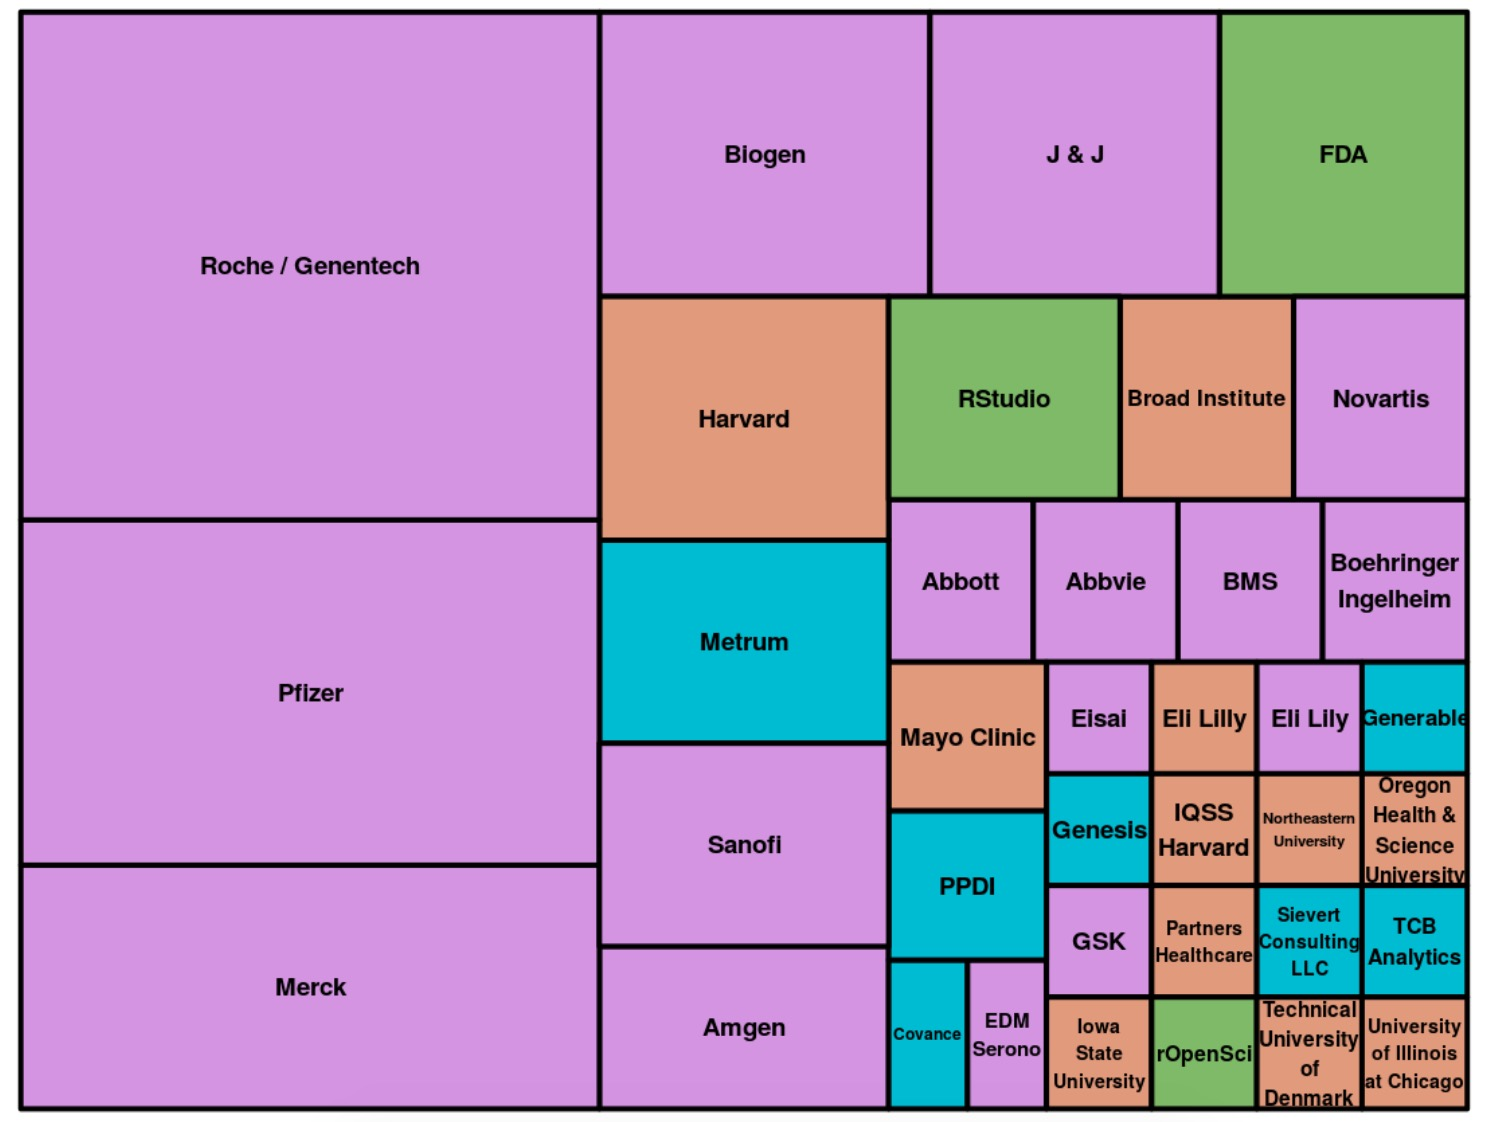
\includegraphics{images/attending.jpg}

\hypertarget{version}{%
\chapter*{Version}\label{version}}


This version of the document was rendered via \texttt{make} at
2018-09-12 15:20:29 by James Black.

The git hash is: 1fe25beeb9bf430413479ded78654f2429c25eaf.

\begin{Shaded}
\begin{Highlighting}[]
\KeywordTok{packageDescription}\NormalTok{(}\StringTok{"bookdown"}\NormalTok{)}\OperatorTok{$}\NormalTok{Version}
\end{Highlighting}
\end{Shaded}

\begin{verbatim}
## [1] "0.7"
\end{verbatim}

\hypertarget{part-overview}{%
\part{Overview}\label{part-overview}}

\hypertarget{schedule}{%
\chapter{Schedule}\label{schedule}}

When

What

Who

Tuesday

18:00 - 21:30

Pre-conference Dinner

Wednesday

07:30 - 09:15

Registration

08:00 - 09:00

Workshop

Keeping things Peachy when Shiny gets Hairy

08:00 - 09:00

Workshop

Analyzing Clinical Trials Data with R

08:00 - 09:00

Workshop

Stan for Pharma

08:00 - 09:00

Workshop

Moving Fast Without Breaking Things: Navigating the R Ecosystem in an
Enterprise Environment

09:15 - 09:25

Opening Remarks

Richard McCullough, Ph.D.~Vice Provost of Research, Harvard University

09:25 - 10:10

Keynote

Modernizing the new drug regulatory program in FDA/CDER: Can
Collaborations and Sharing Help? \textbf{(Lilliam Rosario)}

10:10 - 10:30

Talk

Using R in a regulatory environment: some FDA perspectives \textbf{(Paul
Schuette)}

10:30 - 10:40

Lightning Talk

Using R in a GxP Environment \textbf{(Boyd Gonnerman, et. al.)}

10:40 - 10:50

Lightning Talk

IDBac: A New Paradigm in Developing Microbial Libraries for Drug
Discovery \textbf{(Chase Clark)}

10:50 - 11:10

Break

11:10 - 11:30

Talk

The largest Shiny application in the world. Roche.Diagnostics.bioWARP
\textbf{(Sebastian Wolf)}

11:30 - 11:40

Lightning Talk

R reproducibility by containers and cloud \textbf{(Reinhold Koch)}

11:40 - 11:50

Lightning Talk

Multi-state Model for the Analysis of an Association between Safety and
Efficacy Events \textbf{(Juliane Manitz)}

12:10 - 13:30

Lunch

13:30 - 13:40

Lightning Talk

Becoming bilingual in SAS and R \textbf{(Bella Feng)}

13:40 - 13:50

Lightning Talk

Visualization methods for RNA-sequencing data analysis \textbf{(Lindsay
Rutter)}

13:50 - 14:00

Lightning Talk

The Use of R in the Development of Physiological Model for Healthy
Growth \textbf{(Rena J. Eudy-Byrne)}

14:00 - 14:10

Lightning Talk

Antibody Characterization Using Next Generation Sequencing made easier
with Group My Abs shiny app. \textbf{(Volha Tryputsen)}

14:10 - 14:20

Lightning Talk

Managing R and Associated Tools in Large Environments - an R-Admin's
Perspective \textbf{(Edward Lauzier)}

14:20 - 14:50

Break

14:50 - 15:35

Keynote

Modeling in the tidyverse \textbf{(Max Kuhn)}

15:35 - 15:55

Talk

ShinyRAP - a framework for analysis and building interactive/dynamic
reports using Shiny/Markdown \textbf{(Xiao Ni)}

15:55 - 16:05

Lightning Talk

Data-Driven Strategies for Synthetic Route Design and Operational
Modeling within Pharmaceutical Development \textbf{(Jun Li)}

16:05 - 16:15

Lightning Talk

Evaluating the performance of advanced causal inference methods applied
to healthcare claims data \textbf{(Jessica Myers Franklin)}

16:15 - 16:25

Lightning Talk

Optimization of raw materials genealogy in drug manufacturing with R,
Shiny and d3 \textbf{(Tanya Cashorali)}

16:25 - 16:35

Lightning Talk

REAP - R-Shiny Exploratory Analysis Platform in Clinical Pharmacology
\textbf{(Qi Liu)}

16:35 - 16:45

Lightning Talk

rOpenSci - enabling open and reproducible research \textbf{(Stefanie
Butland)}

17:05 - 17:25

Talk

Beyond Simple Reproducibility - Discoverability, Provenance, and
Improving the Impact of Results \textbf{(Gabe Becker)}

18:00 - 19:30

Reception

Thursday

07:30 - 09:15

Registration

08:00 - 09:00

Workshop

Interactive data visualization with R, plotly, and dashR

08:00 - 09:00

Workshop

The Challenges of Validating R

08:00 - 09:00

Workshop

The largest Shiny application in the world. Roche.Diagnostics.bioWARP

09:15 - 09:25

Opening Remarks

Dustin Tingley, Ph.D., Professor of Government, Harvard University

09:25 - 10:10

Keynote

Using interactivity responsibly in pharma \textbf{(Joe Cheng)}

10:10 - 10:30

Talk

Interactive data visualization with R, plotly, and dashR \textbf{(Carson
Sievert)}

10:30 - 10:50

Talk

Developing powerful Shiny applications in an enterprise environment:
Best practices and lessons learned \textbf{(Eric Nantz)}

10:50 - 11:10

Break

11:10 - 11:30

Talk

NetTCR: Towards Accurate Prediction of T-cell Targets using Deep
Learning \textbf{(Leon Eyrich Jessen)}

11:30 - 11:50

Talk

Analyzing Clinical Trials Data with R \textbf{(Adrian Waddell)}

11:50 - 12:15

Talk

Moving Fast Without Breaking Things: Navigating the R Ecosystem in an
Enterprise Environment \textbf{(Devin Pastoor)}

12:10 - 13:30

Lunch

13:30 - 13:40

Lightning Talk

Unification in a Compartmentalized Culture \textbf{(Mat Soukup)}

13:40 - 13:50

Lightning Talk

R4SPA: R Packages and Training to enable Statistical Programming in R
\textbf{(Kieran Martin)}

13:50 - 14:00

Lightning Talk

Assisting pharmacometric simulation with the use of Shiny \textbf{(Jia
Kang)}

14:00 - 14:10

Lightning Talk

R/Shiny Clinical Dashboards For Fun* and Profit *Note: Fun is Relative
\textbf{(Nate Mockler)}

14:10 - 14:20

Lightning Talk

The drake R package: reproducible data analysis at scale \textbf{(Will
Landau)}

14:20 - 14:50

Break

14:50 - 15:35

Keynote

Enabling open-source analytics in the enterprise \textbf{(Michael
Lawrence)}

15:35 - 15:45

Lightning Talk

The role of R in converting clinical trial programmers to data
scientists \textbf{(James Black)}

15:45 - 15:55

Lightning Talk

Accelerate Personalized Health Care by Empowering Biomarker Data
\textbf{(Xiuting Mi)}

15:55 - 16:05

Lightning Talk

Keeping things Peachy when Shiny gets Hairy \textbf{(Marianna Foos)}

16:05 - 16:15

Lightning Talk

Shiny Apps in Genomics and Clinical Trials \textbf{(Jessica Minnier)}

16:15 - 16:25

Lightning Talk

R as the Core Technology to Support Modeling and Simulation in Pharma
Research, Development, and Post Approval Activities \textbf{(Marc
Gastonquay)}

16:25 - 16:35

Lightning Talk

Building a community of competent developers and users of R-based tools
in mass spectrometry-based research \textbf{(Olga Vitek)}

16:35 - 16:45

Lightning Talk

Bayesian Models for Smaller Trial Sizes \textbf{(Daniel Lee)}

16:45 - 16:55

Lightning Talk

Enhance R Overview \textbf{(Jay Timmerman)}

16:55 - 17:05

Lightning Talk

The Magic R-Shiny App that can Boost your SDTM Usability and Viability
while Saving Time \textbf{(Elma Zannatul Ferdousy \& Katrina Paz)}

17:05 - 17:15

Lightning Talk

Reproducible computational research at Eisai: leadership, technology,
and culture \textbf{(Joseph Gerrein)}

17:15 - 17:25

Lightning Talk

The Challenges of Validating R \textbf{(Andy Nicholls)}

18:00 - 20:00

Informal drinks (not formally organised)

\hypertarget{wednesday}{%
\section{Wednesday}\label{wednesday}}

This is the shortened schedule, please go to
\href{http://rinpharma.com/program/schedule.html}{the Full Schedule} for
more detailed information.

\begin{longtable}[]{@{}lll@{}}
\toprule
\begin{minipage}[b]{0.30\columnwidth}\raggedright
When\strut
\end{minipage} & \begin{minipage}[b]{0.30\columnwidth}\raggedright
What\strut
\end{minipage} & \begin{minipage}[b]{0.30\columnwidth}\raggedright
Slides\strut
\end{minipage}\tabularnewline
\midrule
\endhead
\begin{minipage}[t]{0.30\columnwidth}\raggedright
\textbf{07:30 - 09:15}\strut
\end{minipage} & \begin{minipage}[t]{0.30\columnwidth}\raggedright
\emph{Registration}\strut
\end{minipage} & \begin{minipage}[t]{0.30\columnwidth}\raggedright
\strut
\end{minipage}\tabularnewline
\begin{minipage}[t]{0.30\columnwidth}\raggedright
\textbf{08:00 - 09:00}\strut
\end{minipage} & \begin{minipage}[t]{0.30\columnwidth}\raggedright
\emph{Keeping things Peachy when Shiny gets Hairy (Workshop)}\strut
\end{minipage} & \begin{minipage}[t]{0.30\columnwidth}\raggedright
\strut
\end{minipage}\tabularnewline
\begin{minipage}[t]{0.30\columnwidth}\raggedright
\textbf{08:00 - 09:00}\strut
\end{minipage} & \begin{minipage}[t]{0.30\columnwidth}\raggedright
\emph{Analyzing Clinical Trials Data with R (Workshop)}\strut
\end{minipage} & \begin{minipage}[t]{0.30\columnwidth}\raggedright
\strut
\end{minipage}\tabularnewline
\begin{minipage}[t]{0.30\columnwidth}\raggedright
\textbf{08:00 - 09:00}\strut
\end{minipage} & \begin{minipage}[t]{0.30\columnwidth}\raggedright
\emph{Stan for Pharma (Workshop)}\strut
\end{minipage} & \begin{minipage}[t]{0.30\columnwidth}\raggedright
\strut
\end{minipage}\tabularnewline
\begin{minipage}[t]{0.30\columnwidth}\raggedright
\textbf{08:00 - 09:00}\strut
\end{minipage} & \begin{minipage}[t]{0.30\columnwidth}\raggedright
\emph{Moving Fast Without Breaking Things: Navigating the R Ecosystem in
an Enterprise Environment (Workshop)}\strut
\end{minipage} & \begin{minipage}[t]{0.30\columnwidth}\raggedright
\strut
\end{minipage}\tabularnewline
\begin{minipage}[t]{0.30\columnwidth}\raggedright
\textbf{09:15 - 09:25}\strut
\end{minipage} & \begin{minipage}[t]{0.30\columnwidth}\raggedright
\emph{Opening Remarks}\strut
\end{minipage} & \begin{minipage}[t]{0.30\columnwidth}\raggedright
\strut
\end{minipage}\tabularnewline
\begin{minipage}[t]{0.30\columnwidth}\raggedright
\textbf{09:25 - 10:10}\strut
\end{minipage} & \begin{minipage}[t]{0.30\columnwidth}\raggedright
\emph{Modernizing the new drug regulatory program in FDA/CDER: Can
Collaborations and Sharing Help?}\strut
\end{minipage} & \begin{minipage}[t]{0.30\columnwidth}\raggedright
\strut
\end{minipage}\tabularnewline
\begin{minipage}[t]{0.30\columnwidth}\raggedright
\textbf{10:10 - 10:30}\strut
\end{minipage} & \begin{minipage}[t]{0.30\columnwidth}\raggedright
\emph{Using R in a regulatory environment: some FDA perspectives}\strut
\end{minipage} & \begin{minipage}[t]{0.30\columnwidth}\raggedright
\strut
\end{minipage}\tabularnewline
\begin{minipage}[t]{0.30\columnwidth}\raggedright
\textbf{10:30 - 10:40}\strut
\end{minipage} & \begin{minipage}[t]{0.30\columnwidth}\raggedright
\emph{Using R in a GxP Environment}\strut
\end{minipage} & \begin{minipage}[t]{0.30\columnwidth}\raggedright
\strut
\end{minipage}\tabularnewline
\begin{minipage}[t]{0.30\columnwidth}\raggedright
\textbf{10:40 - 10:50}\strut
\end{minipage} & \begin{minipage}[t]{0.30\columnwidth}\raggedright
\emph{IDBac: A New Paradigm in Developing Microbial Libraries for Drug
Discovery}\strut
\end{minipage} & \begin{minipage}[t]{0.30\columnwidth}\raggedright
\url{https://github.com/chasemc/presentations/blob/master/RinPharma_Aug_2018/rPharma_Chase.pdf}\strut
\end{minipage}\tabularnewline
\begin{minipage}[t]{0.30\columnwidth}\raggedright
\textbf{10:50 - 11:10}\strut
\end{minipage} & \begin{minipage}[t]{0.30\columnwidth}\raggedright
\emph{Break}\strut
\end{minipage} & \begin{minipage}[t]{0.30\columnwidth}\raggedright
\strut
\end{minipage}\tabularnewline
\begin{minipage}[t]{0.30\columnwidth}\raggedright
\textbf{11:10 - 11:30}\strut
\end{minipage} & \begin{minipage}[t]{0.30\columnwidth}\raggedright
\emph{The largest Shiny application in the world.
Roche.Diagnostics.bioWARP}\strut
\end{minipage} & \begin{minipage}[t]{0.30\columnwidth}\raggedright
\strut
\end{minipage}\tabularnewline
\begin{minipage}[t]{0.30\columnwidth}\raggedright
\textbf{11:30 - 11:40}\strut
\end{minipage} & \begin{minipage}[t]{0.30\columnwidth}\raggedright
\emph{R reproducibility by containers and cloud}\strut
\end{minipage} & \begin{minipage}[t]{0.30\columnwidth}\raggedright
\strut
\end{minipage}\tabularnewline
\begin{minipage}[t]{0.30\columnwidth}\raggedright
\textbf{11:40 - 11:50}\strut
\end{minipage} & \begin{minipage}[t]{0.30\columnwidth}\raggedright
\emph{Multi-state Model for the Analysis of an Association between
Safety and Efficacy Events}\strut
\end{minipage} & \begin{minipage}[t]{0.30\columnwidth}\raggedright
\strut
\end{minipage}\tabularnewline
\begin{minipage}[t]{0.30\columnwidth}\raggedright
\textbf{12:10 - 13:30}\strut
\end{minipage} & \begin{minipage}[t]{0.30\columnwidth}\raggedright
\emph{Lunch}\strut
\end{minipage} & \begin{minipage}[t]{0.30\columnwidth}\raggedright
\strut
\end{minipage}\tabularnewline
\begin{minipage}[t]{0.30\columnwidth}\raggedright
\textbf{13:30 - 13:40}\strut
\end{minipage} & \begin{minipage}[t]{0.30\columnwidth}\raggedright
\emph{Becoming bilingual in SAS and R}\strut
\end{minipage} & \begin{minipage}[t]{0.30\columnwidth}\raggedright
\strut
\end{minipage}\tabularnewline
\begin{minipage}[t]{0.30\columnwidth}\raggedright
\textbf{13:40 - 13:50}\strut
\end{minipage} & \begin{minipage}[t]{0.30\columnwidth}\raggedright
\emph{Visualization methods for RNA-sequencing data analysis}\strut
\end{minipage} & \begin{minipage}[t]{0.30\columnwidth}\raggedright
\strut
\end{minipage}\tabularnewline
\begin{minipage}[t]{0.30\columnwidth}\raggedright
\textbf{13:50 - 14:00}\strut
\end{minipage} & \begin{minipage}[t]{0.30\columnwidth}\raggedright
\emph{The Use of R in the Development of Physiological Model for Healthy
Growth}\strut
\end{minipage} & \begin{minipage}[t]{0.30\columnwidth}\raggedright
\strut
\end{minipage}\tabularnewline
\begin{minipage}[t]{0.30\columnwidth}\raggedright
\textbf{14:00 - 14:10}\strut
\end{minipage} & \begin{minipage}[t]{0.30\columnwidth}\raggedright
\emph{Antibody Characterization Using Next Generation Sequencing made
easier with Group My Abs shiny app.}\strut
\end{minipage} & \begin{minipage}[t]{0.30\columnwidth}\raggedright
\strut
\end{minipage}\tabularnewline
\begin{minipage}[t]{0.30\columnwidth}\raggedright
\textbf{14:10 - 14:20}\strut
\end{minipage} & \begin{minipage}[t]{0.30\columnwidth}\raggedright
\emph{Managing R and Associated Tools in Large Environments - an
R-Admin's Perspective}\strut
\end{minipage} & \begin{minipage}[t]{0.30\columnwidth}\raggedright
\strut
\end{minipage}\tabularnewline
\begin{minipage}[t]{0.30\columnwidth}\raggedright
\textbf{14:20 - 14:50}\strut
\end{minipage} & \begin{minipage}[t]{0.30\columnwidth}\raggedright
\emph{Break}\strut
\end{minipage} & \begin{minipage}[t]{0.30\columnwidth}\raggedright
\strut
\end{minipage}\tabularnewline
\begin{minipage}[t]{0.30\columnwidth}\raggedright
\textbf{14:50 - 15:35}\strut
\end{minipage} & \begin{minipage}[t]{0.30\columnwidth}\raggedright
\emph{Modeling in the tidyverse}\strut
\end{minipage} & \begin{minipage}[t]{0.30\columnwidth}\raggedright
\url{http://appliedpredictivemodeling.com/blog/rpharma18}\strut
\end{minipage}\tabularnewline
\begin{minipage}[t]{0.30\columnwidth}\raggedright
\textbf{15:35 - 15:55}\strut
\end{minipage} & \begin{minipage}[t]{0.30\columnwidth}\raggedright
\emph{ShinyRAP - a framework for analysis and building
interactive/dynamic reports using Shiny/Markdown}\strut
\end{minipage} & \begin{minipage}[t]{0.30\columnwidth}\raggedright
\strut
\end{minipage}\tabularnewline
\begin{minipage}[t]{0.30\columnwidth}\raggedright
\textbf{15:55 - 16:05}\strut
\end{minipage} & \begin{minipage}[t]{0.30\columnwidth}\raggedright
\emph{Data-Driven Strategies for Synthetic Route Design and Operational
Modeling within Pharmaceutical Development}\strut
\end{minipage} & \begin{minipage}[t]{0.30\columnwidth}\raggedright
\strut
\end{minipage}\tabularnewline
\begin{minipage}[t]{0.30\columnwidth}\raggedright
\textbf{16:05 - 16:15}\strut
\end{minipage} & \begin{minipage}[t]{0.30\columnwidth}\raggedright
\emph{Evaluating the performance of advanced causal inference methods
applied to healthcare claims data}\strut
\end{minipage} & \begin{minipage}[t]{0.30\columnwidth}\raggedright
\strut
\end{minipage}\tabularnewline
\begin{minipage}[t]{0.30\columnwidth}\raggedright
\textbf{16:15 - 16:25}\strut
\end{minipage} & \begin{minipage}[t]{0.30\columnwidth}\raggedright
\emph{Optimization of raw materials genealogy in drug manufacturing with
R, Shiny and d3}\strut
\end{minipage} & \begin{minipage}[t]{0.30\columnwidth}\raggedright
\url{https://github.com/tcash21/talks/blob/master/TCB\%20Analytics\%20-\%20RPharma\%202018.pdf}\strut
\end{minipage}\tabularnewline
\begin{minipage}[t]{0.30\columnwidth}\raggedright
\textbf{16:25 - 16:35}\strut
\end{minipage} & \begin{minipage}[t]{0.30\columnwidth}\raggedright
\emph{REAP - R-Shiny Exploratory Analysis Platform in Clinical
Pharmacology}\strut
\end{minipage} & \begin{minipage}[t]{0.30\columnwidth}\raggedright
\strut
\end{minipage}\tabularnewline
\begin{minipage}[t]{0.30\columnwidth}\raggedright
\textbf{16:35 - 16:45}\strut
\end{minipage} & \begin{minipage}[t]{0.30\columnwidth}\raggedright
\emph{rOpenSci - enabling open and reproducible research}\strut
\end{minipage} & \begin{minipage}[t]{0.30\columnwidth}\raggedright
\url{https://github.com/ropensci/talks/tree/master/rpharma-2018}\strut
\end{minipage}\tabularnewline
\begin{minipage}[t]{0.30\columnwidth}\raggedright
\textbf{17:05 - 17:25}\strut
\end{minipage} & \begin{minipage}[t]{0.30\columnwidth}\raggedright
\emph{Beyond Simple Reproducibility - Discoverability, Provenance, and
Improving the Impact of Results}\strut
\end{minipage} & \begin{minipage}[t]{0.30\columnwidth}\raggedright
\strut
\end{minipage}\tabularnewline
\begin{minipage}[t]{0.30\columnwidth}\raggedright
\textbf{18:00 - 19:30}\strut
\end{minipage} & \begin{minipage}[t]{0.30\columnwidth}\raggedright
\emph{Reception}\strut
\end{minipage} & \begin{minipage}[t]{0.30\columnwidth}\raggedright
\strut
\end{minipage}\tabularnewline
\bottomrule
\end{longtable}

\hypertarget{thursday}{%
\section{Thursday}\label{thursday}}

This is the shortened schedule, please go to
\href{http://rinpharma.com/program/schedule.html}{the Full Schedule} for
more detailed information.

\begin{itemize}
\tightlist
\item
  \textbf{07:30 - 09:15} \emph{Registration}\\
\item
  \textbf{08:00 - 09:00} \emph{Interactive data visualization with R,
  plotly, and dashR (Workshop)}\\
\item
  \textbf{08:00 - 09:00} \emph{The Challenges of Validating R
  (Workshop)}\\
\item
  \textbf{08:00 - 09:00} \emph{The largest Shiny application in the
  world. Roche.Diagnostics.bioWARP (Workshop)}\\
\item
  \textbf{09:15 - 09:25} \emph{Opening Remarks}\\
\item
  \textbf{09:25 - 10:10} \emph{Using interactivity responsibly in
  pharma}
  \url{https://speakerdeck.com/jcheng5/using-shiny-responsibly-in-pharma}
\item
  \textbf{10:10 - 10:30} \emph{Interactive data visualization with R,
  plotly, and dashR}\\
\item
  \textbf{10:30 - 10:50} \emph{Developing powerful Shiny applications in
  an enterprise environment: Best practices and lessons learned}
  \url{http://rpodcast.gitlab.io/rpharma2018/\#1}
\item
  \textbf{10:50 - 11:10} \emph{Break}\\
\item
  \textbf{11:10 - 11:30} \emph{NetTCR: Towards Accurate Prediction of
  T-cell Targets using Deep Learning}\\
\item
  \textbf{11:30 - 11:50} \emph{Analyzing Clinical Trials Data with R}\\
\item
  \textbf{11:50 - 12:15} \emph{Moving Fast Without Breaking Things:
  Navigating the R Ecosystem in an Enterprise Environment}\\
\item
  \textbf{12:10 - 13:30} \emph{Lunch}\\
\item
  \textbf{13:30 - 13:40} \emph{Unification in a Compartmentalized
  Culture}\\
\item
  \textbf{13:40 - 13:50} \emph{R4SPA: R Packages and Training to enable
  Statistical Programming in R}
  \url{https://kieranjmartin.github.io/R4SPA-talk/r4spa.html\#1}
\item
  \textbf{13:50 - 14:00} \emph{Assisting pharmacometric simulation with
  the use of Shiny}\\
\item
  \textbf{14:00 - 14:10} \_R/Shiny Clinical Dashboards For Fun* and
  Profit *Note: Fun is Relative\_\\
\item
  \textbf{14:10 - 14:20} \emph{The drake R package: reproducible data
  analysis at scale} \url{https://wlandau.github.io/drake-talk/\#/}
\item
  \textbf{14:20 - 14:50} \emph{Break}\\
\item
  \textbf{14:50 - 15:35} \emph{Enabling open-source analytics in the
  enterprise}\\
\item
  \textbf{15:35 - 15:45} \emph{The role of R in converting clinical
  trial programmers to data scientists}
  \url{https://phcanalytics.github.io/slides/aboutus/RinPharma2018/\#/}
\item
  \textbf{15:45 - 15:55} \emph{Accelerate Personalized Health Care by
  Empowering Biomarker Data}\\
\item
  \textbf{15:55 - 16:05} \emph{Keeping things Peachy when Shiny gets
  Hairy}\\
\item
  \textbf{16:05 - 16:15} \emph{Shiny Apps in Genomics and Clinical
  Trials}
  \url{https://jminnier-talks.netlify.com/2018_08_rpharma_shiny/minnier_rpharma2018.html\#1}
\item
  \textbf{16:15 - 16:25} \emph{R as the Core Technology to Support
  Modeling and Simulation in Pharma Research, Development, and Post
  Approval Activities}\\
\item
  \textbf{16:25 - 16:35} \emph{Building a community of competent
  developers and users of R-based tools in mass spectrometry-based
  research}\\
\item
  \textbf{16:35 - 16:45} \emph{Bayesian Models for Smaller Trial
  Sizes}\\
\item
  \textbf{16:45 - 16:55} \emph{Enhance R Overview}\\
\item
  \textbf{16:55 - 17:05} \emph{The Magic R-Shiny App that can Boost your
  SDTM Usability and Viability while Saving Time}\\
\item
  \textbf{17:05 - 17:15} \emph{Reproducible computational research at
  Eisai: leadership, technology, and culture}\\
\item
  \textbf{17:15 - 17:25} \emph{The Challenges of Validating R}\\
\item
  \textbf{18:00 - 20:00} \emph{Informal drinks (not formally organised)}
\end{itemize}

\hypertarget{part-talks}{%
\part{Talks}\label{part-talks}}

\hypertarget{keynotes}{%
\chapter{Keynotes}\label{keynotes}}

To start viewing abstracts, either 1) press right on your keyboard, 2)
click the arrow or 3) select a talk from the menu.

\hypertarget{modernizing-the-new-drug-regulatory-program-in-fdacder-can-collaborations-and-sharing-help}{%
\section{\texorpdfstring{\emph{Modernizing the new drug regulatory
program in FDA/CDER: Can Collaborations and Sharing
Help?}}{Modernizing the new drug regulatory program in FDA/CDER: Can Collaborations and Sharing Help?}}\label{modernizing-the-new-drug-regulatory-program-in-fdacder-can-collaborations-and-sharing-help}}

\textbf{Lilliam Rosario}, FDA Center for Drug Evaluation \& Research

\emph{Wednesday, 15th August from 09:25 - 10:10}

Lilliam will be presenting a perspective on what the office of
computational science is doing to support regulatory review for safety
assessments. She will explore the concept of collaborations and sharing
to support process and transparency, along with a perspective with the
use of R.

\hypertarget{modeling-in-the-tidyverse}{%
\section{\texorpdfstring{\emph{Modeling in the
tidyverse}}{Modeling in the tidyverse}}\label{modeling-in-the-tidyverse}}

\textbf{Max Kuhn}, RStudio

\emph{Wednesday, 15th August from 14:50 - 15:35}

The tidyverse (tidyverse.org) is an opinionated collection of R packages
designed for data science. All packages share an underlying design
philosophy, grammar, and data structures. The packages primarily consist
of tools for data ingest, manipulation, and visualization. In the last
year or so, Rstudio and others have been creating a set of packages
focused on the modeling process. In this talk, we will introduce the
tidyverse and illustrate these new tools whose goals are to: simplify
the modeling process, encourage empirical validation and good
methodology, and to enable a wider variety of approaches.

\hypertarget{using-interactivity-responsibly-in-pharma}{%
\section{\texorpdfstring{\emph{Using interactivity responsibly in
pharma}}{Using interactivity responsibly in pharma}}\label{using-interactivity-responsibly-in-pharma}}

\textbf{Joe Cheng}, RStudio

\emph{Thursday, 16th August from 09:25 - 10:10}

Shiny is a package for turning analyses written in R into interactive
web applications. This capability has obvious applications in pharma, as
it lets R users build interactive apps for their collaborators to
explore models or results, or to automate workflows. However, the
interactivity of Shiny apps is a double-edged sword, as it introduces
challenges to the traceability and reproducibility of your analysis. To
use interactive applications in pharma responsibly, these challenges
must be addressed. In this talk, I'll look at some of the tools and
techniques you can use in Shiny to deal with these challenges head-on.

\hypertarget{enabling-open-source-analytics-in-the-enterprise}{%
\section{\texorpdfstring{\emph{Enabling open-source analytics in the
enterprise}}{Enabling open-source analytics in the enterprise}}\label{enabling-open-source-analytics-in-the-enterprise}}

\textbf{Michael Lawrence}, Genentech, R Core Team

\emph{Thursday, 16th August from 14:50 - 15:35}

The open-source analytics community is driving innovation in
precompetitive spaces like statistical methodology, reproducibility
approaches, visualization techniques, and scaling strategies. The
diverse and rapdily evolving ecosystem of open-source tools and
standards stands in contrast with the disposition of the enterprise
towards stability, standardization, and reliability. This talk will
present the policies and frameworks we have developed at Genentech to
enable internal scientists to responsibly leverage open-source tools and
to participate in the community process through their own contributions.

\hypertarget{talks---by-author}{%
\chapter{Talks - by author}\label{talks---by-author}}

To start viewing abstracts, either 1) press right on your keyboard, 2)
click the arrow or 3) select a talk from the menu.

\hypertarget{analyzing-clinical-trials-data-with-r}{%
\section{\texorpdfstring{\emph{Analyzing Clinical Trials Data with
R}}{Analyzing Clinical Trials Data with R}}\label{analyzing-clinical-trials-data-with-r}}

\textbf{Adrian Waddell}, Roche

\emph{Thursday, 16th August from 11:30 - 11:50}

Creating datasets and tables, listings and graphs (TLGs) for analyzing
clinical trials data with R, such that in the final stage the code,
datasets and TLGs can be submitted to the health authorities, is a
multifaceted problem. We have been working on a number of R packages to
create an R-based analysis environment that can be used for exploratory
and regulatory analysis of clinical trials data. These projects include:
table creation (open source \url{http://github.com/Roche/rtables});
random data generation; querying CDISC standards; TLG creation; a
pipeline for specifying and producing data and TLG deliverables (with
logs, automation, titles and footnotes, etc.); a modular shiny-based
exploratory framework that provides dynamic encodings, variable-based
filtering, and R-code generation for the displayed outputs. The maturity
of these projects varies, but the workflow and analysis environment as a
whole can be demonstrated nicely. In this talk, we would like to
generate interest in collaboration in order to make these projects more
general and with the final goal of open-sourcing some of them.

\hypertarget{the-challenges-of-validating-r}{%
\section{\texorpdfstring{\emph{The Challenges of Validating
R}}{The Challenges of Validating R}}\label{the-challenges-of-validating-r}}

\textbf{Andy Nicholls}, GlaxoSmithKline

\emph{Thursday, 16th August from 17:15 - 17:25}

The first challenge in validating an analytic tool for the
pharmaceutical industry is that, despite a formal FDA definition, there
is still no cross-industry agreement on what `validation' really means
with respect to an analytic tool. AIMS (Application and Implementation
of Methodologies in Statistics), a Special Interest Group within PSI
have been attempting to answer this question with respect to R. In doing
so we recently received approval from the R Consortium for an online R
package validation repository and are now looking to formalise some
early definitions. In this presentation I will walk through some of the
challenges that we have identified thus far and outline what we're
hoping to achieve with the platform.

\hypertarget{becoming-bilingual-in-sas-and-r}{%
\section{\texorpdfstring{\emph{Becoming bilingual in SAS and
R}}{Becoming bilingual in SAS and R}}\label{becoming-bilingual-in-sas-and-r}}

\textbf{Bella Feng}, Amgen

\emph{Wednesday, 15th August from 13:30 - 13:40}

In this talk, I will speak about my personal journey of learning R and
transforming from a clinical study statistical programmer to a SAS/R
bilingual, as well as my journey of leading the R initiative in Amgen's
Global Statistical Programming Department and Amgen R meetup, working
with IS, statistician, quality, LMS and external partners. I will
conclude by talking about the areas of challenge and the direction of R
for statistical programming in a regulated environment and proposals for
R in Pharma collaboration.

\hypertarget{using-r-in-a-gxp-environment}{%
\section{\texorpdfstring{\emph{Using R in a GxP
Environment}}{Using R in a GxP Environment}}\label{using-r-in-a-gxp-environment}}

\textbf{Boyd Gonnerman, John Sims, Frank DePierro and Peter Giardina},
Pfizer

\emph{Wednesday, 15th August from 10:30 - 10:40}

The Data Science team in Pfizer's Vaccine Research and Development
division (VRD) creates and maintains validated applications used during
high-throughput clinical testing that enable advanced analytic and
reporting requirements. SAS has long been the de-facto standard for
analyzing data in a regulated GxP environment. Web deployment of these
applications has been the best approach, and Pfizer VRD has developed
several mid-tier applications in Java that submit batch SAS processes on
a High Performance Computing grid. Pfizer VRD's high level approach is
the same across different assay platforms: data are pulled from a
combination of electronic files and Oracle databases and analyzed,
results are written back to an Oracle database, and electronic output
files are made in various formats (e.g.~PDF). The regulated nature of
Pfizer VRD's work and the difficulty in deploying R-based applications
over the web have previously been an impediment to the use of R, but new
tools such as RStudio's Shiny Server Pro have helped us overcome those
challenges. This presentation focuses on a comparison of the
architecture used to deploy our SAS applications and the infrastructure
required to deploy R-based applications to meet GxP requirements. Real
life examples will be provided to illustrate the usefulness of this
platform in a regulated laboratory environment.

\hypertarget{interactive-data-visualization-with-r-plotly-and-dashr}{%
\section{\texorpdfstring{\emph{Interactive data visualization with R,
plotly, and
dashR}}{Interactive data visualization with R, plotly, and dashR}}\label{interactive-data-visualization-with-r-plotly-and-dashr}}

\textbf{Carson Sievert}, Sievert Consulting

\emph{Thursday, 16th August from 10:10 - 10:30}

Interactive web graphics are a popular and convenient medium for
conveying information. However, web graphics are rarely used during the
initial exploratory phase of a data analysis, largely due to the lack
tools for seamless iteration between data manipulation, modeling, and
visualization. As we've known for several decades, interactive graphics
can augment exploratory analysis, but are only practical when we can
iterate quickly. This talk demonstrates how to use the R packages plotly
and dashR to rapidly produce interactive web graphics and applications
that augment data exploration in addition to being easily distributed.

\hypertarget{idbac-a-new-paradigm-in-developing-microbial-libraries-for-drug-discovery}{%
\section{\texorpdfstring{\emph{IDBac: A New Paradigm in Developing
Microbial Libraries for Drug
Discovery}}{IDBac: A New Paradigm in Developing Microbial Libraries for Drug Discovery}}\label{idbac-a-new-paradigm-in-developing-microbial-libraries-for-drug-discovery}}

\textbf{Chase Clark}, Student, University of Illinois at Chicago

\emph{Wednesday, 15th August from 10:40 - 10:50}

The success of a bacterial drug discovery program can be no greater than
the phylogenetic diversity and capacity of those bacteria in the library
to produce specialized metabolites (SM). However, the methods used to
create bacterial strain libraries have seen little innovation in nearly
80 years. Current practice relies entirely on colony morphology and/or
16S rRNA gene sequencing analysis to decide which isolated strains to
retain for addition to a drug discovery library. However, these
practices create inefficient libraries plagued with a high degree of
taxonomic and chemical redundancy by relying on physical characteristics
that have limited correlation with strains' SM, the foundation of drug
discovery. Therefore, the development of a platform to rapidly
prioritize unknown bacterial strains based on phylogeny and SM would
greatly increase the efficiency of the front-end of microbial drug
discovery. Our lab has recently developed such a platform, called IDBac,
which uses in situ matrix-assisted laser desorption/ionization
time-of-flight mass spectrometry (MALDI-TOF MS) to analyze protein and
specialized metabolite spectra of single bacterial colonies. Utilizing R
and Shiny, alongside state-of-the-art packages and techniques in MALDI
processing and data visualization, we created a stand-alone executable
program for MALDI-TOF MS bacterial analysis. Using unsupervised learning
methods and visualizations we have demonstrated IDBac's capabilities by
creating protein and specialized metabolite MS profiles, generating
protein MS hierarchical groupings that accurately mirrored phylogenetic
groupings and further distinguishing isolates based on inter- and
intra-species differences in specialized metabolite production. With the
ease of use of modern MALDI instrumentation and interactive, intuitive
data exploration, IDBac can rapidly profile up to 384 bacteria in 4
hours. To our knowledge, IDBac is the first attempt to couple in situ MS
analyses of protein content and specialized metabolite production and
will enable laboratories with access to a MALDI-TOF MS the ability to
rapidly create more efficient libraries for their drug discovery
programs.

\hypertarget{bayesian-models-for-smaller-trial-sizes}{%
\section{\texorpdfstring{\emph{Bayesian Models for Smaller Trial
Sizes}}{Bayesian Models for Smaller Trial Sizes}}\label{bayesian-models-for-smaller-trial-sizes}}

\textbf{Daniel Lee}, Generable

\emph{Thursday, 16th August from 16:35 - 16:45}

Precision medicine typically refers to the development of drugs and
other interventions for individual patients. But how do you assess
efficacy and make predictions in this extreme small data regime?

The Bayesian framework is ideal for this type of inference as it allows
us to combine population and personal effects in a principled way and
make predictions for both groups and individuals. The inferences are
further improved when we introduce mechanistically inspired components
into the modeling framework.

I'll talk about building pharma models in the small data regime and how
we use Stan (a statistical modeling language for Bayesian inference)
with R for analysis.

\hypertarget{moving-fast-without-breaking-things-navigating-the-r-ecosystem-in-an-enterprise-environment}{%
\section{\texorpdfstring{\emph{Moving Fast Without Breaking Things:
Navigating the R Ecosystem in an Enterprise
Environment}}{Moving Fast Without Breaking Things: Navigating the R Ecosystem in an Enterprise Environment}}\label{moving-fast-without-breaking-things-navigating-the-r-ecosystem-in-an-enterprise-environment}}

\textbf{Devin Pastoor}, Metrum Research Group

\emph{Thursday, 16th August from 11:50 - 12:15}

Despite the explosive growth and adoption of R globally, concerns over
how to qualify and administrate R continues to echo in discussions about
use in regulated environments. In this talk, I'll discuss the how to
bridge the conceptual tenants of reproducibility, traceability, and
accuracy to robust, yet agile, implementations such that and
organization can maintain validated systems without imposing the
shackles found in traditional validated environments. Furthermore, I
will discuss a number of design elements specific to the open-source R
ecosystem, such as using packages from CRAN and github, and cover how to
embrace these, while responsibly managing risk in enterprise
environments.

\hypertarget{managing-r-and-associated-tools-in-large-environments---an-r-admins-perspective}{%
\section{\texorpdfstring{\emph{Managing R and Associated Tools in Large
Environments - an R-Admin's
Perspective}}{Managing R and Associated Tools in Large Environments - an R-Admin's Perspective}}\label{managing-r-and-associated-tools-in-large-environments---an-r-admins-perspective}}

\textbf{Edward Lauzier}, Merck

\emph{Wednesday, 15th August from 14:10 - 14:20}

The dramatic increase of R in the computational, analytics, and data
science areas has led to some innovative techniques in recent years for
interactive analytics. This rate of change presents challenges for IT
organizations to keep up and to maintain their software stacks for
scientists for regulated and non-regulated environments. Techniques and
Best Practices for managing updates and use cases will be presented from
an R-Admin's perspective using a combination of opensource and
professional tools.

\hypertarget{the-magic-r-shiny-app-that-can-boost-your-sdtm-usability-and-viability-while-saving-time}{%
\section{\texorpdfstring{\emph{The Magic R-Shiny App that can Boost your
SDTM Usability and Viability while Saving
Time}}{The Magic R-Shiny App that can Boost your SDTM Usability and Viability while Saving Time}}\label{the-magic-r-shiny-app-that-can-boost-your-sdtm-usability-and-viability-while-saving-time}}

\textbf{Elma Zannatul Ferdousy, Katrina Paz and Nasser Al Ali },
Genetech

\emph{Thursday, 16th August from 16:55 - 17:05}

The United States Food and Drug Administration (FDA) requires that
clinical trial data be submitted in the Study Data Tabulation Model
(SDTM) standard format. The process of developing SDTM involves mapping
captured raw data to their correspondent SDTM domains based on rules and
conditions put by the Clinical Data Interchange Standards Consortium
(CDISC) organization. SDTM data is further used for building the
Analysis Data Model (ADaM) which is used for clinical trial statistical
analysis. Mistakes in the mapping process are common due to the process
complexities; issues that are missed may potentially affect the clinical
trial result. Therefore, it is very essential to preserve the quality of
the SDTM data. Currently, the main tool for checking SDTM conformance is
Pinnacle21 (formerly known as OpenCDISC). Notably, there are usability
and viability checks that are not included in Pinnacle21. This work
describes the creation of an R shiny app to supplement the Pinnacle21
checks. This interactive app applies various CDISC-compliant SDTM data
validation checks, and provides the user with a comprehensive report on
possible inconsistencies in the data. The app would allow programmers to
proactively find data mapping errors. In addition, it is straightforward
to use and can save tremendous amounts of time. Additionally, this app's
audience extends beyond the programming community and covers other
individuals who have an interest in data quality, particularly Data
Managers and individuals in Clinical Science and Clinical Operations.

\hypertarget{developing-powerful-shiny-applications-in-an-enterprise-environment-best-practices-and-lessons-learned}{%
\section{\texorpdfstring{\emph{Developing powerful Shiny applications in
an enterprise environment: Best practices and lessons
learned}}{Developing powerful Shiny applications in an enterprise environment: Best practices and lessons learned}}\label{developing-powerful-shiny-applications-in-an-enterprise-environment-best-practices-and-lessons-learned}}

\textbf{Eric Nantz}, Lilly

\emph{Thursday, 16th August from 10:30 - 10:50}

Recent advances in the Shiny ecosystem boost the scale and scope of
serious enterprise-wide web applications. More specifically, it is
entirely possible to utilize key features of Shiny Server Professional
and additional R packages such as shinyjs, DT, and batchtools to build
Shiny applications that supports session management, high-performance
computing, and reproducibility in a friendly and logical interface.
Additionally, the shinytest package enables a robust workflow for
developing applications efficiently, as well as being an important
component to automate a validation testing framework. In this talk, I
will share examples of key features and lessons learned in creating a
technically powerful shiny application that integrates these pieces
together.

\hypertarget{beyond-simple-reproducibility---discoverability-provenance-and-improving-the-impact-of-results}{%
\section{\texorpdfstring{\emph{Beyond Simple Reproducibility -
Discoverability, Provenance, and Improving the Impact of
Results}}{Beyond Simple Reproducibility - Discoverability, Provenance, and Improving the Impact of Results}}\label{beyond-simple-reproducibility---discoverability-provenance-and-improving-the-impact-of-results}}

\textbf{Gabe Becker}, Genentech

\emph{Wednesday, 15th August from 17:05 - 17:25}

Research is an incremental, iterative process, with new results relying
and building upon previous ones. Scientists need to find, retrieve,
understand, and trust results in order to confidently extend them, even
when the results are their own. We present the GREX framework, which
facilitates this iterative process via the principled management of
computational results. GREX combines robust storage, provenance
tracking, automated annotation, discoverability, and reproduciblity of
computational results. We will discuss both the underlying conceptual
work and our reference implementation of our framework.

\hypertarget{the-role-of-r-in-converting-clinical-trial-programmers-to-data-scientists}{%
\section{\texorpdfstring{\emph{The role of R in converting clinical
trial programmers to data
scientists}}{The role of R in converting clinical trial programmers to data scientists}}\label{the-role-of-r-in-converting-clinical-trial-programmers-to-data-scientists}}

\textbf{James Black}, Roche

\emph{Thursday, 16th August from 15:35 - 15:45}

In 3 years Real World Data Science Analytics in Roche/Genentech
transitioned from a small team of former clinical trial programmers
supporting a real world evidence team to become the largest department
within the Personalised Healthcare (PHC) Centre of Excellence. This
transition was driven by industry-wide acknowledgement of the growing
importance of leveraging analytics to support PHC, but this change
necessitated radical changes in workflows and competencies. To adapt to
this change, the team has moved from using a single proprietary software
(SAS) to becoming an open source-focused, R based but increasingly
programming language agnostic, department. A core driver of this
transition was the development of an internal suite of R packages that
handled markdown templates and database access through to wrappers for
common plots and documenting git hashes of all code used. Bringing this
diverse set of tools into a coherent eco-system is a meta-package
modelled on the tidyverse.

\hypertarget{enhance-r-overview}{%
\section{\texorpdfstring{\emph{Enhance R
Overview}}{Enhance R Overview}}\label{enhance-r-overview}}

\textbf{Jay Timmerman}, Covance

\emph{Thursday, 16th August from 16:45 - 16:55}

Recruitment models for clinical trials are notoriously difficult to
build due to many complex factors within a study. With input from
experienced practitioners, we have built an interactive tool to allow
individuals to build complex recruitment models using the R/Shiny
framework. The Tool Enhance R, our platform for study modeling, was
ported from an Excel-based tool to the R/Shiny platform to increase
model development speed, expand capability and drive transparency into
model development. The tool allows users to specify critical model
attributes (i.e.~country site distribution, recruitment/activation
rates, country-specific vacations), and provide instantaneous feedback
that changes have on a model's probability of success. Using the RStudio
Connect platform, we are able to grant multi-level access to users
through a single web interface. Model development is tracked by
exporting results to a SharePoint site and logging versions for future
review/auditing. This gives significant levels of transparency on how a
model was created and evolved over time. For web analytics, we used
Piwik, and internal web analytics platform, to monitor how users
navigate through the platform and identify browsing behavior. The
application was built upon the Shiny Dashboard framework and leverages
many visualization packages, including Plotly, Timevis, ggplot2 and many
more. Many challenges arose in its develop, from controlling
over-zealous user clicks causing out of control execution, to
integrating service account execution of apps to facilitate centralized
data control. This project pushed the limits of what the R/Shiny
platform is capable of and demonstrates how data scientists can build
useful solutions.

\hypertarget{shiny-apps-in-genomics-and-clinical-trials}{%
\section{\texorpdfstring{\emph{Shiny Apps in Genomics and Clinical
Trials}}{Shiny Apps in Genomics and Clinical Trials}}\label{shiny-apps-in-genomics-and-clinical-trials}}

\textbf{Jessica Minnier}, Oregon Health \& Science University (OHSU)

\emph{Thursday, 16th August from 16:05 - 16:15}

R Shiny has revolutionized the way statisticians and analysts distribute
analytic results and research methods. We can easily build interactive
web tools that enhance data visualization and facilitate data and
information sharing. Shiny apps can empower non-statisticians to explore
and visualize their data or perform their own analyses with methods we
develop. Harnessing this power, R users have developed Shiny apps for
visualizing clinical trials and pharmaceutical data, as well as
applications that aid in study design and analysis. I will present
examples of how Shiny can be used in many stages of the drug development
process and discuss the challenges as well as benefits of incorporating
these tools in pharmaceutical workflows.

\hypertarget{evaluating-the-performance-of-advanced-causal-inference-methods-applied-to-healthcare-claims-data}{%
\section{\texorpdfstring{\emph{Evaluating the performance of advanced
causal inference methods applied to healthcare claims
data}}{Evaluating the performance of advanced causal inference methods applied to healthcare claims data}}\label{evaluating-the-performance-of-advanced-causal-inference-methods-applied-to-healthcare-claims-data}}

\textbf{Jessica Myers Franklin}, Harvard Medical School, Brigham and
Women's Hospital

\emph{Wednesday, 15th August from 16:05 - 16:15}

Cohort studies of treatments developed from healthcare claims often have
hundreds of thousands of patients and up to several thousand measured
covariates. Therefore, new causal inference methods that combine ideas
from machine learning and causal inference may improve analysis of these
studies by taking advantage of the wealth of information measured in
claims. In order to evaluate the performance of these methods as applied
to claims-based studies, we use a combination of real data examples and
plasmode simulation, implemented in R package `plasmode', which creates
realistic simulated datasets based on a real cohort study. In this talk,
I will give an overview of our progress so far and what is left to be
done.

\hypertarget{assisting-pharmacometric-simulation-with-the-use-of-shiny}{%
\section{\texorpdfstring{\emph{Assisting pharmacometric simulation with
the use of
Shiny}}{Assisting pharmacometric simulation with the use of Shiny}}\label{assisting-pharmacometric-simulation-with-the-use-of-shiny}}

\textbf{Jia Kang }, Metrum Research Group

\emph{Thursday, 16th August from 13:50 - 14:00}

During the drug development, pharmacometric models are often built to
characterize and understand drug efficacy and safety. Simulations based
on these models can assist drug development and quantitative decision
making. However, computation can be time-consuming and communication
with the project team may not be productive. Shiny applications are
developed as a simulation tool which allows rapid real-time simulations
based on user-selected inputs and dynamic visualization of the results.
It provides an easy access to individuals with no specific background of
modeling and simulation. In the talk, I will present some case studies
where the shiny application was used to perform simulations and
facilitate the communication with decision makers.

\hypertarget{reproducible-computational-research-at-eisai-leadership-technology-and-culture}{%
\section{\texorpdfstring{\emph{Reproducible computational research at
Eisai: leadership, technology, and
culture}}{Reproducible computational research at Eisai: leadership, technology, and culture}}\label{reproducible-computational-research-at-eisai-leadership-technology-and-culture}}

\textbf{Joseph Gerrein}, Eisai

\emph{Thursday, 16th August from 17:05 - 17:15}

The pharmaceutical industry depends on accurate and reproducible data
science for both preclinical and clinical analysis. Unfortunately, often
an analysis cannot be reproduced and therefore its computational
methodology and merit are unknown. Often, the data, code, or description
of computational methods is not maintained. In order to implement good
practices of reproducible computational research, the leadership of the
company must invest time and resources into planning, training, ensuring
adoption of common practices and tools, implementing documentation
systems, encouraging discipline on the individual and group level,
creating incentives, and requiring accountability. At Eisai, we have
developed a working system for reproducible computational research that
is enabled by leadership, technology, and culture. With regards to
technology, we primarily use Rmarkdown and R Notebooks on an Rstudio
server used by all our analysts. The Rstudio server is maintained by an
administrator who installs packages for all users, creating a common
package environment that ensures that code can be rerun in the future.
Data and code are stored in a shared network drive and version control
is accomplished by using Git. A wiki that is editable by all analysts is
used to organize all analyses (tracked with unique analysis IDs) and
provides links to code and results.

With regards to culture, the leadership has promoted the values of
quality and reproducibility. When yearly objectives are set, the
performance criteria includes the creation of analysis documents
(e.g.~Rmarkdown reports), use of version control, and organization of
data on shared network drives. Setting aside time for wiki documentation
in the midst of high demands from project teams is helped by having
periodic ``documentation day'' parties. To verify reproducibility, we
have implemented ``witnessing'': once the analysis is finished, it is
reviewed by an independent team member who officially signs off on the
work, stating that the reproducibility criteria have been met. Our
success in implementing reproducible computational research can serve as
a model for other companies to use. Here we have provided a model based
on leadership, technology, and culture.

\hypertarget{multi-state-model-for-the-analysis-of-an-association-between-safety-and-efficacy-events}{%
\section{\texorpdfstring{\emph{Multi-state Model for the Analysis of an
Association between Safety and Efficacy
Events}}{Multi-state Model for the Analysis of an Association between Safety and Efficacy Events}}\label{multi-state-model-for-the-analysis-of-an-association-between-safety-and-efficacy-events}}

\textbf{Juliane Manitz}, EMD Serono

\emph{Wednesday, 15th August from 11:40 - 11:50}

Safety and efficacy data in clinical trials are mostly analyzed
separately. However, especially the treatment of life-threatening
disease such as cancer requires a good understanding of benefit and
associated risks to make an informed therapy decision for an individual
patient. Recently approved immunotherapeutic drugs in oncology are
associated with potential side effects such as immune-related
hypothyroidism, rash and colitis. There is some biological reasoning
that the occurrence of immune-related adverse events and corresponding
management may compromise the drug response. On the other hand, it has
been observed that patients responding to treatment might face a higher
likelihood of adverse drug reactions. A multi-state model is able to
explore these hypotheses and offers the opportunity of insights into
potential associations while addressing some of the methodological
challenges. For example, the necessity of a time-dependent approach to
accommodate the fact that safety and efficacy events can occur
throughout the treatment. Moreover, longer treatment duration can impact
simultaneously the likelihood of efficacy as well as safety events,
i.e., introducing immortal time bias. The multistate model is able to
unfold this spurious correlation. We present an approach for analysis
and exemplify the methodology with simulated data.

\hypertarget{data-driven-strategies-for-synthetic-route-design-and-operational-modeling-within-pharmaceutical-development}{%
\section{\texorpdfstring{\emph{Data-Driven Strategies for Synthetic
Route Design and Operational Modeling within Pharmaceutical
Development}}{Data-Driven Strategies for Synthetic Route Design and Operational Modeling within Pharmaceutical Development}}\label{data-driven-strategies-for-synthetic-route-design-and-operational-modeling-within-pharmaceutical-development}}

\textbf{Jun Li}, Bristol Myers Squibb

\emph{Wednesday, 15th August from 15:55 - 16:05}

Decision analysis balancing both data analytics and human gut feeling is
critical in designing efficient routes to synthesize new, complex small
molecules. This challenge is faced by any organization seeking to
deliver modern pharmaceutical compounds to patients in a prompt manner.
In this presentation, we highlight the incorporation of data science
approaches using R to develop metrics that aid in the development
process: current complexity, risk quantification, and process efficiency
forecasting. Current complexity is a metric established from human
insights that assesses a molecule's complexity in the context of
capability, tracking the `current' complexity of a given molecule over
time and enabling the quantitative assessment of a new route or process.
Risk quantification utilizes a Bayesian framework to quantify risk from
real data and operational patterns, at both the project and portfolio
level, for assessing the delivery risk of early candidate nomination
assets in areas such as FTE resource modeling. Process efficiency can be
estimated with a predictive analytics framework capable of quantifying
the probable efficiency of a proposed synthesis or benchmarking the
outcome performance of the developed process, thereby minimizing the
environmental impact of pharmaceutical production. These strategies have
been effectively used to aid the decision-making processes for
pharmaceutical R\&D.

\hypertarget{r4spa-r-packages-and-training-to-enable-statistical-programming-in-r}{%
\section{\texorpdfstring{\emph{R4SPA: R Packages and Training to enable
Statistical Programming in
R}}{R4SPA: R Packages and Training to enable Statistical Programming in R}}\label{r4spa-r-packages-and-training-to-enable-statistical-programming-in-r}}

\textbf{Kieran Martin}, Roche

\emph{Thursday, 16th August from 13:40 - 13:50}

R is a very powerful tool for performing statistical programming, but
has had a lower uptake in the life sciences when compared to SAS. As a
result, many of the packages created for R are not focused on the type
of tasks Statistical Programmers do. In this talk I introduce several
packages and in house training we are developing to aid regulatory
outputs. The R packages include rcompare, a package to allow comparison
of datasets, analogous to proc compare in SAS, and r4spa which allows
outputs to be in the correct format for production. Each package solves
a problem particular to the life sciences, and is intended to improve
uptake of R usage within the industry. Similarly, to the R packages, the
training is focused on providing examples of actual work, so that users
of the training will be able to immediately apply their knowledge.

\hypertarget{nettcr-towards-accurate-prediction-of-t-cell-targets-using-deep-learning}{%
\section{\texorpdfstring{\emph{NetTCR: Towards Accurate Prediction of
T-cell Targets using Deep
Learning}}{NetTCR: Towards Accurate Prediction of T-cell Targets using Deep Learning}}\label{nettcr-towards-accurate-prediction-of-t-cell-targets-using-deep-learning}}

\textbf{Leon Eyrich Jessen}, DTU Technical University of Denmark

\emph{Thursday, 16th August from 11:10 - 11:30}

Vanessa Isabell Jurtz(1), Leon Eyrich Jessen(1), Martin Closter
Jespersen(1), Kamilla Kjærgaard Jensen(1), Bjoern Peters(2), Paolo
Marcatili(1), Morten Nielsen(1). (1). Department of Bio and Health
Informatics, Technical University of Denmark, Lyngby, Denmark. (2). La
Jolla Institute for Allergy and Immunology, San Diego, California, USA.

The interaction between the Major Histocompatibility Complex type I
(MHC-I), a peptide and the T-cell receptor (TCR) (MHCI::p::TCR) is a key
determinant of immune response elicitation and therefore of paramount
importance in infectious- and autoimmune diseases and cancer. Current
state-of-the-art models developed by our group can with great precision
model MHCI::p interactions. Using data from VDJdb and IEDB, we created
an ensemble of convolutional neural networks, which to the best of our
knowledge is the world's first sequence based model capable of capturing
the entire MHCI::p::TCR system. Due to limited data, we however
currently can only model the interaction between the CDR3 region of the
TCR's beta chain with HLA-A*02:01 and 3 peptides. However, as the model
framework is easily extendable, we will increase the breadth and thus
improve the model, as soon as more data become available. Using the
current model and an independent test set, we obtained AUC = 0.747.

TensorFlow is an open source software library for neural network models
made by Google. Recently RStudio released Keras an API for accessing
TensorFlow in R. Keras enables fast experimentation - Being able to go
from idea to result with the least possible delay is key to doing good
research.

\hypertarget{visualization-methods-for-rna-sequencing-data-analysis}{%
\section{\texorpdfstring{\emph{Visualization methods for RNA-sequencing
data
analysis}}{Visualization methods for RNA-sequencing data analysis}}\label{visualization-methods-for-rna-sequencing-data-analysis}}

\textbf{Lindsay Rutter}, Iowa State University

\emph{Wednesday, 15th August from 13:40 - 13:50}

RNA-seq data is biased and accurate detection of differentially
expressed genes (DEGs) is not a trivial task. While the data collection
can be considered high-throughput, data analysis has intricacies that
require careful human attention. The most effective approach to modern
data analysis is to iterate between models and visuals, and to enhance
the appropriateness of models based on feedback from visuals. As it
stands, there is a need to make it easier for scientists and clinicians
to use models and visuals in a complimentary fashion during RNA-seq data
analysis. Here, we use public RNA-seq data to show that our
visualization tools can detect normalization problems, DEG designation
problems, and common errors in RNA-seq analysis. We also show that our
tools can identify genes of interest that cannot be obtained with
models. Through this project, we propose that users slightly modify
their approach to data analysis by quickly assessing the sensibility of
their models with statistical graphics. We plan to publish a new R
software package that includes the plotting techniques introduced in
this project, which can be useful for exploring several types of
multivariate biological data such as RNA-sequencing data.

\hypertarget{r-as-the-core-technology-to-support-modeling-and-simulation-in-pharma-research-development-and-post-approval-activities}{%
\section{\texorpdfstring{\emph{R as the Core Technology to Support
Modeling and Simulation in Pharma Research, Development, and Post
Approval
Activities}}{R as the Core Technology to Support Modeling and Simulation in Pharma Research, Development, and Post Approval Activities}}\label{r-as-the-core-technology-to-support-modeling-and-simulation-in-pharma-research-development-and-post-approval-activities}}

\textbf{Marc Gastonquay}, Metrum Research Group

\emph{Thursday, 16th August from 16:15 - 16:25}

Since its foundation in 2004, Metrum Research Group has relied on R as
the core technology and central framework for all of the company's
biomedical modeling and simulation (M\&S) service activities, spanning
more than 475 projects with 150+ different sponsors. Projects include
pharmacokinetic-pharmacodynamic modeling, quantitative systems
pharmacology models, simulation-based trial design evaluations, disease
progression and patient population modeling, model-based meta analysis
of competitor data, model-based comparative effectiveness assessments,
and data management activities, etc., all within a regulated
environment. Analyses were conducted in R or via other software tools
which are managed via R scripts, functions, or packages. Key
deliverables of M\&S projects are routinely provided as R packages or
interactive simulation applications, driven by R (and R Shiny). R has
also been an essential component of Metrum's vision for Open Science in
biomedical M\&S, allowing for accessibility and reproducibility of
platform models developed for multiple disease areas.

\hypertarget{keeping-things-peachy-when-shiny-gets-hairy}{%
\section{\texorpdfstring{\emph{Keeping things Peachy when Shiny gets
Hairy}}{Keeping things Peachy when Shiny gets Hairy}}\label{keeping-things-peachy-when-shiny-gets-hairy}}

\textbf{Marianna Foos}, Biogen

\emph{Thursday, 16th August from 15:55 - 16:05}

Shiny is a popular R package that lets users develop interactive web
applications using just R code. The ease of use and downstream boost in
productivity mean that working with Shiny can kick off a rapid
request-implementation-inspiration-request cycle. Designing your
applications with an eye toward future expansion can save time and
reduce human error in the long term.

\hypertarget{unification-in-a-compartmentalized-culture}{%
\section{\texorpdfstring{\emph{Unification in a Compartmentalized
Culture}}{Unification in a Compartmentalized Culture}}\label{unification-in-a-compartmentalized-culture}}

\textbf{Mat Soukup}, FDA

\emph{Thursday, 16th August from 13:30 - 13:40}

When it comes to analytics of data collected in medical research,
today's culture is compartmentalized -- not only across institutions,
but even within institutions. Such a culture stagnates analytical
development and limits the ability to fully master the data thereby
reducing the effectiveness in communicating clinical information to
stakeholders. A unified culture can exist -- statisticians, programmers,
and clinicians need to speak to each other; regulatory agencies,
pharmaceutical companies, and academics need to speak to each other.
Once everyone comes together to discuss how the medical research data
should be collected, interrogated and presented; analytics can be
developed and shared within and across institutions. From an analytics
perspective, nothing new needs to be developed, solutions are already
available -- many of them free. We just need to come together and start
talking. So let's talk.

\hypertarget{rshiny-clinical-dashboards-for-fun-and-profit-note-fun-is-relative_}{%
\section{\_R/Shiny Clinical Dashboards For Fun* and Profit *Note: Fun is
Relative\_}\label{rshiny-clinical-dashboards-for-fun-and-profit-note-fun-is-relative_}}

\textbf{Nate Mockler}, Biogen

\emph{Thursday, 16th August from 14:00 - 14:10}

For the Pharma Company How many times have you made a graph and gotten
an email back saying: ``Can we change the axes?'' or ``Can we change the
symbols?'' or ``I really need to look at the graph before I can tell you
what I want''. It would be much more efficient for your customers to
explore the data and the visualizations in an easy-to-use method and can
free you up to work on the myriad other tasks you have to do. Rather
than learn another programming language, the shiny package uses the R
code you already know to create interactive visualizations with a small
bit of additional learning. This talk will go over example dashboards
for such data as adverse events, labs, and primary endpoints that will
aid data managers, statisticians, clinical people, and\ldots{} even you.

\hypertarget{building-a-community-of-competent-developers-and-users-of-r-based-tools-in-mass-spectrometry-based-research}{%
\section{\texorpdfstring{\emph{Building a community of competent
developers and users of R-based tools in mass spectrometry-based
research}}{Building a community of competent developers and users of R-based tools in mass spectrometry-based research}}\label{building-a-community-of-competent-developers-and-users-of-r-based-tools-in-mass-spectrometry-based-research}}

\textbf{Olga Vitek}, Northeastern University

\emph{Thursday, 16th August from 16:25 - 16:35}

The R-based ecosystem, and its open-source methods for data
manipulation, modeling and interpretation, is key for effective and
reproducible research. This is certainly true in experiments relying on
quantitative mass spectrometry. This relatively new and rapidly evolving
field must overcome many sources of unwanted variation. It has many
unsolved challenges, both in the appropriate use of the existing methods
and tools, and in developing methods that address specialized problems.

This talk will illustrate our R-based efforts to promote sound
statistical practice, and build a community of competent practitioners.
First, we will present Cardinal, a comprehensive tool for quantitative
mass spectrometry-based imaging, as well as MSstats, a general but
flexible framework for mass spectrometry-based proteomics. We will
highlight the importance of these tools for pharmaceutical research in
an example of statistical characterization of therapeutic protein
modifications. Second, we will detail our efforts of building a
community of competent users through a world-wide series of short
courses, intended for experimentalists and computational scientists
alike.

\hypertarget{using-r-in-a-regulatory-environment-some-fda-perspectives}{%
\section{\texorpdfstring{\emph{Using R in a regulatory environment: some
FDA
perspectives}}{Using R in a regulatory environment: some FDA perspectives}}\label{using-r-in-a-regulatory-environment-some-fda-perspectives}}

\textbf{Paul Schuette}, FDA

\emph{Wednesday, 15th August from 10:10 - 10:30}

The United States Food and Drug Administration (FDA) uses a variety of
statistical software packages for review and research. This presentation
will focus on the uses of R in the Center for Drug Evaluation and
Research (CDER), including graphics for labels, Bayesian designs and
analyses, simulations, machine learning, data quality and data integrity
efforts, as well as interactive visualizations using R Shiny. Some of
the challenges with using R will be discussed, as well as advantages of
using R to collaborate with colleagues in industry and academe through
Cooperative Research and Development Agreements (CRADAs), Broad Agency
Agreements (BAAs), and working groups associated with professional
societies (ASA, DIA, PhUSE).

\hypertarget{reap---r-shiny-exploratory-analysis-platform-in-clinical-pharmacology}{%
\section{\texorpdfstring{\emph{REAP - R-Shiny Exploratory Analysis
Platform in Clinical
Pharmacology}}{REAP - R-Shiny Exploratory Analysis Platform in Clinical Pharmacology}}\label{reap---r-shiny-exploratory-analysis-platform-in-clinical-pharmacology}}

\textbf{Qi Liu}, Genentech

\emph{Wednesday, 15th August from 16:25 - 16:35}

Qi Liu, Christopher Wen, Scott Pivirotto, Jin Jin, Matts Kagedal
Genentech, Inc., South San Francisco, CA, USA

REAP (R-Shiny Exploratory Analysis Platform) was developed by the
Modeling and Simulation group within the Clinical Pharmacology
department at Genentech, Inc., to support exploratory analyses of
clinical data. REAP is a web-based, user-friendly, tool providing
standard methods and outputs for conducting typical analyses within a
clinical pharmacology group. With REAP, a clinical pharmacologist or
pharmacometrician can perform Exposure-Response, dose linearity, and
concentration-corrected QT analyses, PKPD simulations, NONMEM data
quality checks, and PK graphic analyses without writing code. Results
can be used to enhance scientific understanding of the relationship
between exposure, response, and the PK characteristics of the molecule.
In this talk, I will demonstrate how REAP can be used to perform dose
linearity and Exposure-Response analyses.

\hypertarget{r-reproducibility-by-containers-and-cloud}{%
\section{\texorpdfstring{\emph{R reproducibility by containers and
cloud}}{R reproducibility by containers and cloud}}\label{r-reproducibility-by-containers-and-cloud}}

\textbf{Reinhold Koch}, Roche

\emph{Wednesday, 15th August from 11:30 - 11:40}

R is pretty good in backwards compatibility but still reproducing
analysis even given script and data can be a challenge as packages, R,
and math libraries keep evolving. www.rocker-project.org offers among
other things version-stable R in docker (Rocker) images. A small example
will be presented how this allows on any docker runtime environment to
execute analysis with highest reproducibility. Such environments are
part of all major commercial cloud providers but also allow on-premises
installations.

\hypertarget{the-use-of-r-in-the-development-of-physiological-model-for-healthy-growth}{%
\section{\texorpdfstring{\emph{The Use of R in the Development of
Physiological Model for Healthy
Growth}}{The Use of R in the Development of Physiological Model for Healthy Growth}}\label{the-use-of-r-in-the-development-of-physiological-model-for-healthy-growth}}

\textbf{Rena J. Eudy-Byrne}, Metrum Research Group

\emph{Wednesday, 15th August from 13:50 - 14:00}

A physiologically-based mathematical model was developed as a series of
ordinary differential equations to describe compositional changes (in
fat and fat-free mass, FM \& FFM) due to metabolizable energy exchanges
in babies from birth to 2 years in low-to-middle income countries.1 The
objective of this work was to identify potential biomarkers for future
intervention studies, identify when to intervene to protect and/or
rescue growth in individuals suffering from malnutrition, and to
identify which of these individuals would be more or less likely to
respond to a nutritional intervention.

A translation of this model (155 parameters and 26 compartments) using R
and the open-source mrgsolve package2 provided an efficient platform for
multi-parameter optimization, as required during additional model
development and for subsequent simulations. For comparison, a 8.62
seconds simulation with viral and bacterial infections (no
interventions) in the R/mrgsolve implementation required 226 seconds in
Matlab. Model translation to R also enabled simulations with a Shiny
App, allowing users to simulate individual infant phenotypes and
infection events and visualize growth and energy levels over time,
relative to healthy (WHO) standards.

The model currently also includes a relatively simple implementation of
persistent antibiotic therapy with a potential for inclusion of drug
exposure-related effects, i.e. - through a pharmacokinetic (PK) model,
to describe effects of antiviral or antibiotic therapy. The challenge to
this development is the scarcity of available data describing this
therapy in malnourished children that would be needed for model
calibration. Further development of the model includes linking to other
systems models such Mother-fetus energy exchange or PBPK mother-fetus
models, to enable simulations of growth beginning at gestation.

References: 1.) Bill \& Melinda Gates Foundation Healthy birth, growth
and development knowledge integration (HBGDki) project provided access
to data and also funded this work. Model was developed by Mike Morimoto
and Lyn Powell. 2.) Kyle T Baron (2018). mrgsolve: Simulate from
ODE-Based Population PK/PD and Systems Pharmacology Models. R package
version 0.8.12.https://CRAN.R-project.org/package=mrgsolve

\hypertarget{the-largest-shiny-application-in-the-world.-roche.diagnostics.biowarp}{%
\section{\texorpdfstring{\emph{The largest Shiny application in the
world.
Roche.Diagnostics.bioWARP}}{The largest Shiny application in the world. Roche.Diagnostics.bioWARP}}\label{the-largest-shiny-application-in-the-world.-roche.diagnostics.biowarp}}

\textbf{Sebastian Wolf}, Roche

\emph{Wednesday, 15th August from 11:10 - 11:30}

bioWARP (biostatistical Web-Applications and R Procedures) is a Shiny
application enabling employees at Roche Diagnostics to create validated
reports for regulatory authorities submissions. bioWARP enables people
using advanced statistical methods, who cannot program R. It builds a
connection to the validated R-packages developed at Roche with an easy
to use and elegant user interface. Its modular environment can host an
unlimited number of such interfaces. bioWARP now consists of tools for
reporting reference ranges, equality by linear regression, precision by
variance component analysis and homogeneity by inhouse developed
equivalence tests . bioWARP's most important feature is the ability to
move all statistical evaluations right into PDF reports. These are
validated and can directly be used for submission to regulatory
authorities. bioWARP is called the ``largest shiny application in the
world'' by us as it already consists of 16 tools, has over 100.000 lines
of code, \textgreater{}500 buttons and interaction items and is growing
and growing and growing.

\hypertarget{ropensci---enabling-open-and-reproducible-research}{%
\section{\texorpdfstring{\emph{rOpenSci - enabling open and reproducible
research}}{rOpenSci - enabling open and reproducible research}}\label{ropensci---enabling-open-and-reproducible-research}}

\textbf{Stefanie Butland}, rOpenSci

\emph{Wednesday, 15th August from 16:35 - 16:45}

The rOpenSci project is a non-profit initiative founded as a grassroots
effort in 2011. We have evolved into a truly global community of
researchers and data scientists who are R users and developers from a
wide range of disciplines. rOpenSci advocates for a culture of open and
reproducible research. We do this by creating technical infrastructure
in the form of carefully vetted, staff- and community-contributed R
software tools that lower barriers to working with scientific data
sources on the web. We have developed a highly successful model for peer
review of scientific software that provides transparent, constructive
and collegial review of R packages.

Our community is our best asset. We are building social infrastructure
in the form of a welcoming and diverse community. rOpenSci.org hosts
blog posts by authors and reviewers of onboarded packages to share both
functionality and lessons learned; we promote these on social media to
bring their work to a wider audience. Our discussion forum, community
calls and annual hackathon-flavored unconference are designed to share
best practices and to build a trust network for the often challenging
discussions about doing research more reproducibly.

\hypertarget{optimization-of-raw-materials-genealogy-in-drug-manufacturing-with-r-shiny-and-d3}{%
\section{\texorpdfstring{\emph{Optimization of raw materials genealogy
in drug manufacturing with R, Shiny and
d3}}{Optimization of raw materials genealogy in drug manufacturing with R, Shiny and d3}}\label{optimization-of-raw-materials-genealogy-in-drug-manufacturing-with-r-shiny-and-d3}}

\textbf{Tanya Cashorali}, TCB Analytics

\emph{Wednesday, 15th August from 16:15 - 16:25}

Failure to thoroughly review discrepancies and deviations in drug
manufacturing is consistently one of the top citations in FDA
inspectional observations. Learn how a leading biotechnology
organization successfully replaced an inefficient, manual inspection
process with a genealogy visualization and inspection solution to
optimize drug manufacturing quality control. This session will cover
implementation approaches and lessons learned in data mapping,
technology selection, visualization development, and predictive model
generation.

\hypertarget{antibody-characterization-using-next-generation-sequencing-made-easier-with-group-my-abs-shiny-app.}{%
\section{\texorpdfstring{\emph{Antibody Characterization Using Next
Generation Sequencing made easier with Group My Abs shiny
app.}}{Antibody Characterization Using Next Generation Sequencing made easier with Group My Abs shiny app.}}\label{antibody-characterization-using-next-generation-sequencing-made-easier-with-group-my-abs-shiny-app.}}

\textbf{Volha Tryputsen}, Johnson \& Johnson

\emph{Wednesday, 15th August from 14:00 - 14:10}

Next-generation sequencing (NGS), phage display technology and high
throughput capacities enables biologists in drug discovery to
characterize antibodies (Abs) based on their HCDR3 sequences and further
group them into families before moving to hit-to-lead stage of drug
discovery and development. This enables diversification of Ab portfolio
and insures back up options if Ab candidate fails. However, there was no
method or software available in-house to support Ab discovery with
capacities to apply biophysical rules to classify the sequences. Shiny
app ``Group My Abs'' was developed to apply biophysical properties for
Ab characterization to the NGS data. Several Multiple Sequence Alignment
algorithms implemented in the app enable sequence comparability. A
method was developed to evaluate differences between comparable
sequences and subsequently classify sequences into families. The app
provides custom-made and interactive data visualization, enables refined
Ab classification in a mathematical manner, considerably increases
efficiency and insures reproducibility. This all decreases bias and
enables informative decision making during the hit-to-lead stage in
biologics drug discovery.

\hypertarget{the-drake-r-package-reproducible-data-analysis-at-scale}{%
\section{\texorpdfstring{\emph{The drake R package: reproducible data
analysis at
scale}}{The drake R package: reproducible data analysis at scale}}\label{the-drake-r-package-reproducible-data-analysis-at-scale}}

\textbf{Will Landau}, Lilly

\emph{Thursday, 16th August from 14:10 - 14:20}

The drake package is a general-purpose workflow manager for data-driven
tasks in R, with applications in the pharmaceutical industry ranging
from tailored medicine to clinical trial simulation and beyond. Drake
rebuilds intermediate data objects when their dependencies change, and
it skips work when the results are already up to date. Not every
runthrough starts from scratch, and completed workflows have tangible
evidence of reproducibility. Drake is more scalable than knitr, more
thorough than memoization, and more R-focused than other pipeline
toolkits such as GNU Make, remake, and snakemake.

\hypertarget{shinyrap---a-framework-for-analysis-and-building-interactivedynamic-reports-using-shinymarkdown}{%
\section{\texorpdfstring{\emph{ShinyRAP - a framework for analysis and
building interactive/dynamic reports using
Shiny/Markdown}}{ShinyRAP - a framework for analysis and building interactive/dynamic reports using Shiny/Markdown}}\label{shinyrap---a-framework-for-analysis-and-building-interactivedynamic-reports-using-shinymarkdown}}

\textbf{Xiao Ni}, Novartis

\emph{Wednesday, 15th August from 15:35 - 15:55}

R has become a prominent data science tool, empowered by a fast-growing
modern R eco-system. At Novartis, Shiny and markdown have gained a lot
of popularity in analyzing, visualizing and reporting of clinical trial
data. Traditional report analysis plan (RAP) process was designed to
create static table, figure and listings. In this talk, I will use
ShinyRAP (a shiny app) to illustrate a novel framework/workflow of
planning and executing of both pre-specified and ad-hoc analyses, as
well as building dynamic/interactive reports through R/Shiny/Markdown.
The app features efficient and organized programming through meta-data
and shiny modules, and dynamic display of results via multi-select,
grouping and searching, etc. Although motivated from a clinical trial
data context, this framework can also be used for other types of data.

\hypertarget{accelerate-personalized-health-care-by-empowering-biomarker-data}{%
\section{\texorpdfstring{\emph{Accelerate Personalized Health Care by
Empowering Biomarker
Data}}{Accelerate Personalized Health Care by Empowering Biomarker Data}}\label{accelerate-personalized-health-care-by-empowering-biomarker-data}}

\textbf{Xiuting Mi}, Roche

\emph{Thursday, 16th August from 15:45 - 15:55}

In Pharmaceutical industry, personalized patient care is about having
access to traditional and new data sources including comprehensive
diagnostic data, sensor data, real-world data, etc., applying
traditional and advanced analytics like machine learning to create
meaningful insights, and then realizing value from those insights for
smarter and more efficient research and development (R\&D) and improving
patient access and personalized patient care. Biomarker research is a
key component of the PHC Strategy, complementing efforts to access
high-dimensional genomics data and conducting appropriated analysis
using right tools differentiate from those for current well-established
clinical trials. This paper, in perspective of R\&D, describes the close
collaboration between China Oncology Biomarker Data group (OBD China)
and Product Development Biometrics (PDB) expertise, from sample
collection, lab process in biomarker stand-alone studies to meaningful
results mainly conducted in R, which enables to prioritize molecule
development, inform the design of specific trials and identify R\&D
opportunities for regional diseases.

\hypertarget{summary-plots}{%
\chapter{Summary plots}\label{summary-plots}}

Following section provides summary information about the conference.

\hypertarget{attendees}{%
\section{Attendees}\label{attendees}}

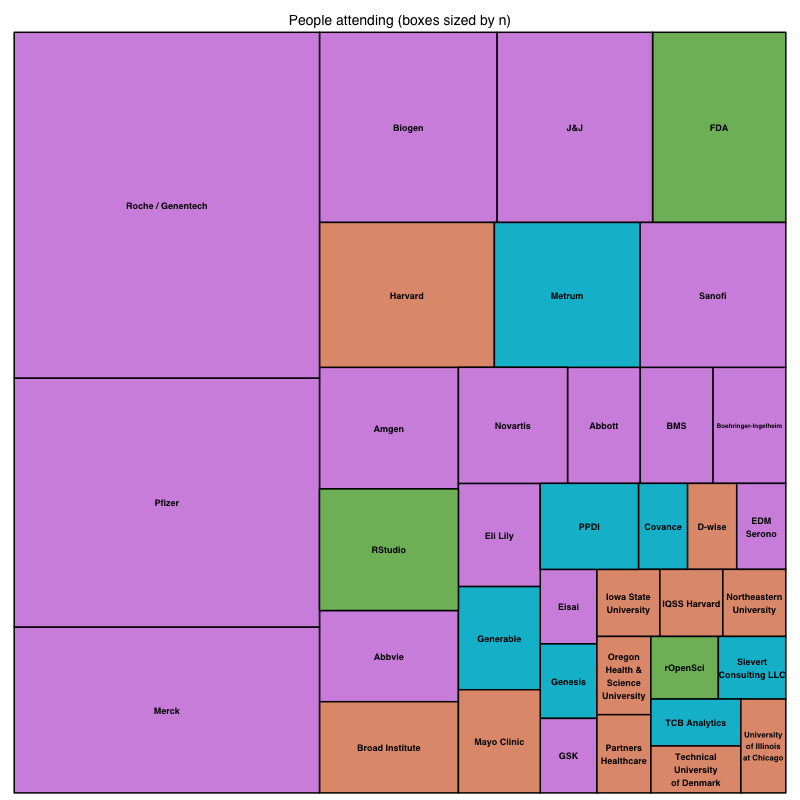
\includegraphics{tree.png}

\hypertarget{wordclouds}{%
\section{Wordclouds}\label{wordclouds}}

A wordcloud based on speaker abstracts

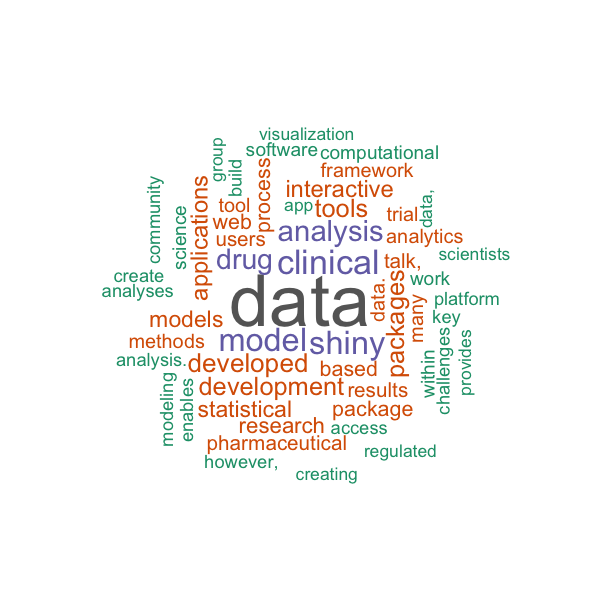
\includegraphics{wc_abstracts.png}

A wordcloud based on speaker presentation titles

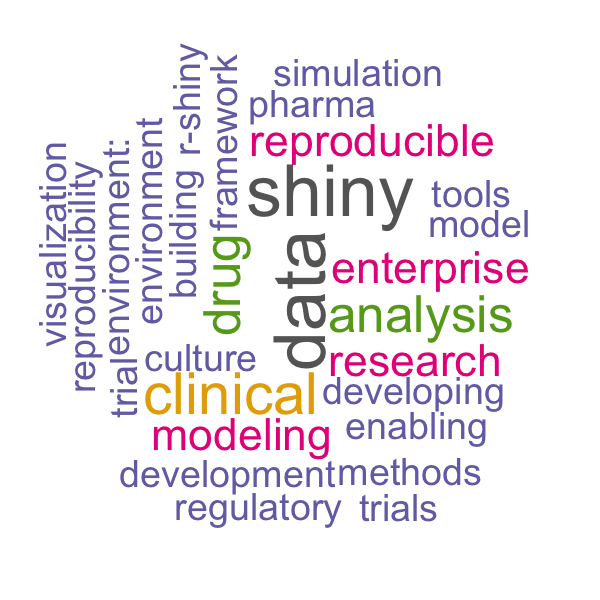
\includegraphics{wc_titles.png}A wordcloud based on companies present

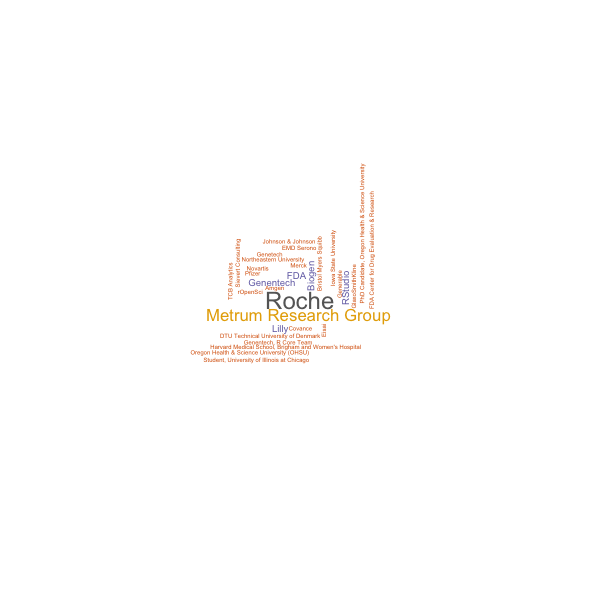
\includegraphics{wc_comps.png}

\backmatter
\printindex

\end{document}
